\section{Evaluation \label{sec:evaluation}}

This chapter explain the divers evaluation metrics used and experiments realized on the datasets to evaluate the proposed methods (ref. Section~\ref{sec:methods}).

\subsection{Rank lists}

\subsubsection{Rank list evaluation metrics}
\label{sec:rl_eval}

In order to know the quality of a rank list, the following metrics are used.
Definitions in this sections are an adapted version of the ones in Kocher and Savoy's \textit{Evaluation of text representation schemes and distance measures for authorship linking}~\cite{kocher_linking}.
The presented metrics are well know in the authorship verification and the information retrieval field.

\begin{definition}[Relevant link~\cite{kocher_linking}]
  A relevant link is a link in the relevant set.
  The relevant set is explain in Definition~\ref{def:relevant_set}.
  \begin{equation}
    relevant(l_i) =
    \begin{cases}
      1, & if\ l_i \in R \\
      0, & otherwise
    \end{cases}
  \end{equation}
\end{definition}

\begin{definition}[Precision@k~\cite{kocher_linking}]
  The precision@k is a function which take a positive integer k, with k < |L|
  \begin{equation}
    precision(k) = \frac{1}{k} \sum_{j=1}^{k} relevant(j)
  \end{equation}
\end{definition}

\begin{definition}[Average Precision (AP)]
  The mean over the precision@k each time a relevant link is retrieved.
  \begin{equation}
    AveragePrecision = \frac{1}{|R|} \sum_{j=1}^{|L|} precision(j) \cdot relevant(j)
  \end{equation}
  The average precision can be considered as an approximation of the area under the precision-recall curve.
\end{definition}

\begin{definition}[R-Precision~\cite{kocher_linking}]
  The R-Precision (RPrec) is the precision in the rank list at rank |R| (Precision@r).
  With R being the relevant set (Definition~\ref{def:relevant_set}).
  \begin{equation}
    RPrec = precision(|R|)
  \end{equation}
  The RPrec value is in the range $\left[0, 1\right]$.
  With 0 mean every links in the first $|R|$-ranks are not in the relevant set.
  And 1, every links in the first $|R|$-ranks are in the relevant set.
\end{definition}

\begin{definition}[High precision~\cite{kocher_linking}]
  The high precision (HPrec) represent the maximal rank j in the rank list such that the precision is still 100\%.
  \begin{equation}
    HPrec = \max\{i \in \mathbf{N} | precision(i) = 1\}
  \end{equation}
  This value is in the range $\left[0, |R|\right]$.
  $0$ means the first pair in the rank list is incorrect.
  $|R|$ means every true links are ranked in the top part of the rank list.
\end{definition}

\subsubsection{Importance of the text size in stylometry}

Previous studies have shown the importance of having documents of good quality and with at least 5000 tokens to have reliable results.
Skilled authors can easily change their style to imitate others for small texts, but it becomes more difficult for larger texts~\cite{savoy_stylo}.

For this study, an experiment on the St-Jean dataset is accomplish, in the order to show the importance of having large documents.
In order to test this parameter, the number of token is artificially modified by considering only the $n$ first tokens for each text, with $n$ ranging between 9000 and 250 with steps of 250 tokens.

Figure~\ref{img:degradation} shows the three metrics used (Average precision, RPrec, HPrec) over the number of tokens.
Every metrics decrease over the text size, which indicate that it becomes harder to determinate documents pairs with the same author as the text size decrease.

\begin{figure}
  \centering
  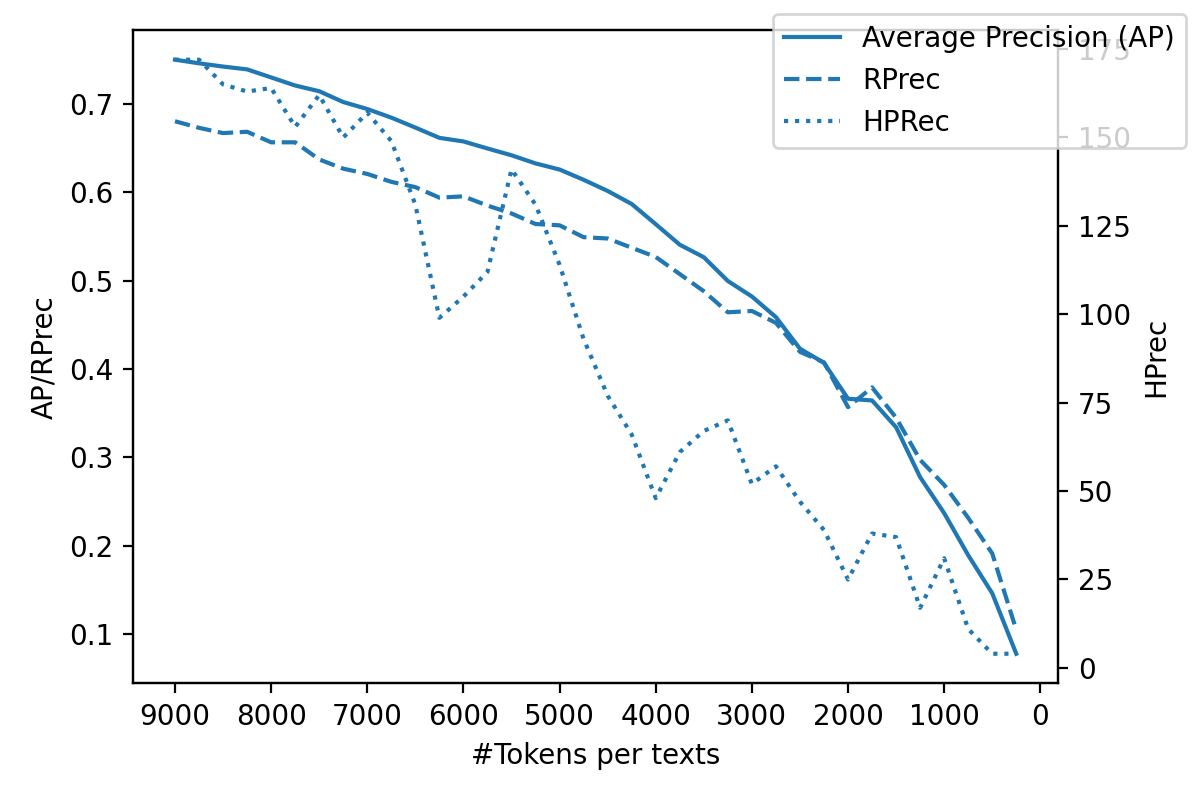
\includegraphics[width=\linewidth]{img/degradation.png}
  \caption{St-Jean ranks list evaluation on AP, RPrec and HPrec over the text size. Rank list computed using 500 MFW and the zscored-normalized cosine distance}
  \label{img:degradation}
\end{figure}

PAN16 dataset is a difficult dataset due to its small size, thus extracting reliable features for each text to estimate each style is also a difficult task.
After multiple tests, the PAN @ CLEF 2016 dataset is not used further in this study due to its difficulty in finding reliable Stylometric clues.

\subsubsection{MFW Token and Lemma}

Here the goal is to compare two similar text representations, which are the token representation, words as they can appear in the novels, and the lemmatize representation, for example \textit{il voit} (he sees) will be lemmatized to \textit{il voir} (he see).
For this kind of representation, previous studies have shown that using MFW (most frequent words) vector size of around 500 tends to produce better outcomes~\cite{savoy_text_representation}.

After creating the rank lists with the proposed distance measures (ref. Section~\ref{sec:fv_distances}) on the two representations for a MFW vector size ranging between 100 and 2000 with a step of 100, on the two datasets containing the lemmatize representation (Brunet and St-Jean), the two plots in Figure~\ref{fig:token_vs_lemma} show the average precision (AP) for the resulting rank lists.

This representation seem to have good results with a MFW vector size of 500 for most of the metrics, this corroborate previous studies results.
A few metrics, such as the Manhattan distance or the Clark distance can give better results with slightly bigger vectors.
In most cases, the token representation provide on both dataset a greater average precision compared to the lemma representation.
An interesting example to be worth noticing concern the Manhattan distance, when using the token representation it tends to decrease the AP faster than the lemma representation as the MFW vector size increase.
The euclidean distance seem to be the least appropriate distance measure for this task.
The Clark distance have a really poor average precision when the MFW vector is too small but after reaching 500 it produces one of the best pay-off of the experiment.
Over all, the cosine distance seem to be one of the most appropriate choice when dealing with these datasets and text representations.

\begin{figure}
  \caption{Token and Lemma representation over number of MFW using different distances metrics}
  \label{fig:token_vs_lemma}

  \subcaption{Brunet}
  \label{fig:token_vs_lemma_brunet}
  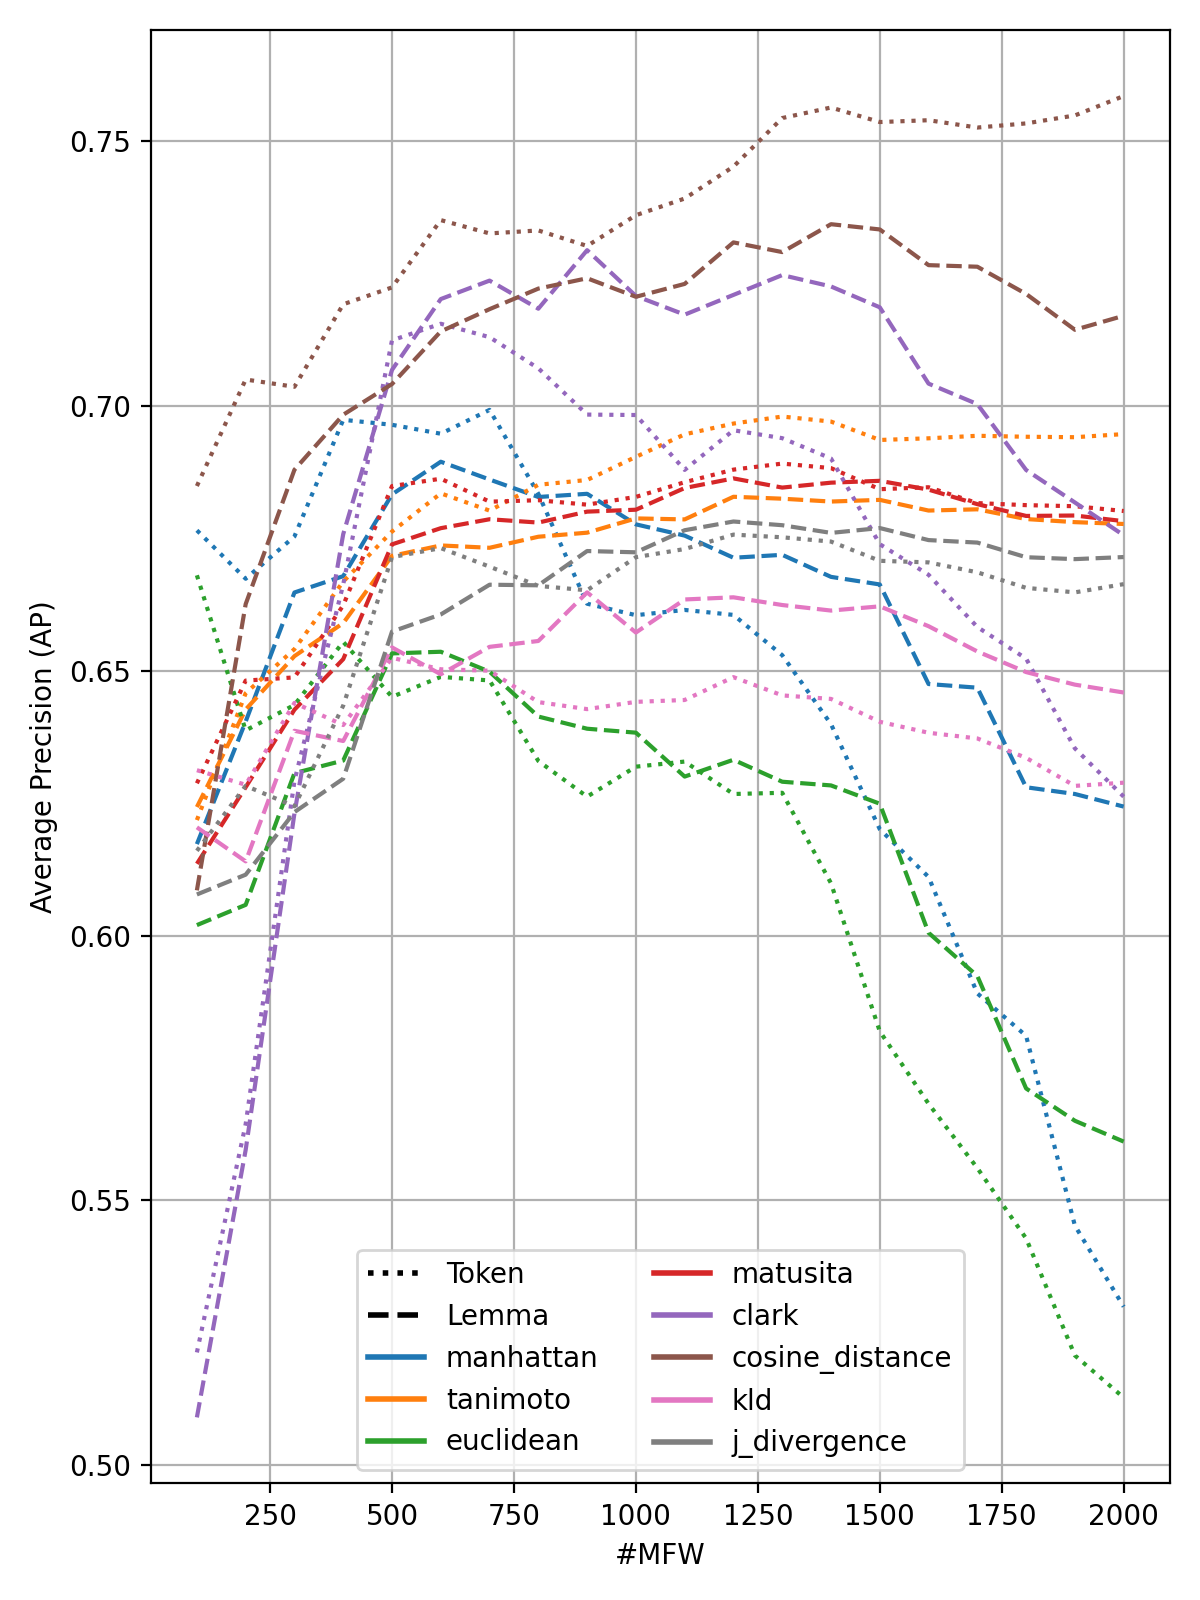
\includegraphics[width=0.9\linewidth]{img/token_vs_lemma_brunet.png}

  \subcaption{St-Jean}
  \label{fig:token_vs_lemma_st_jean}
  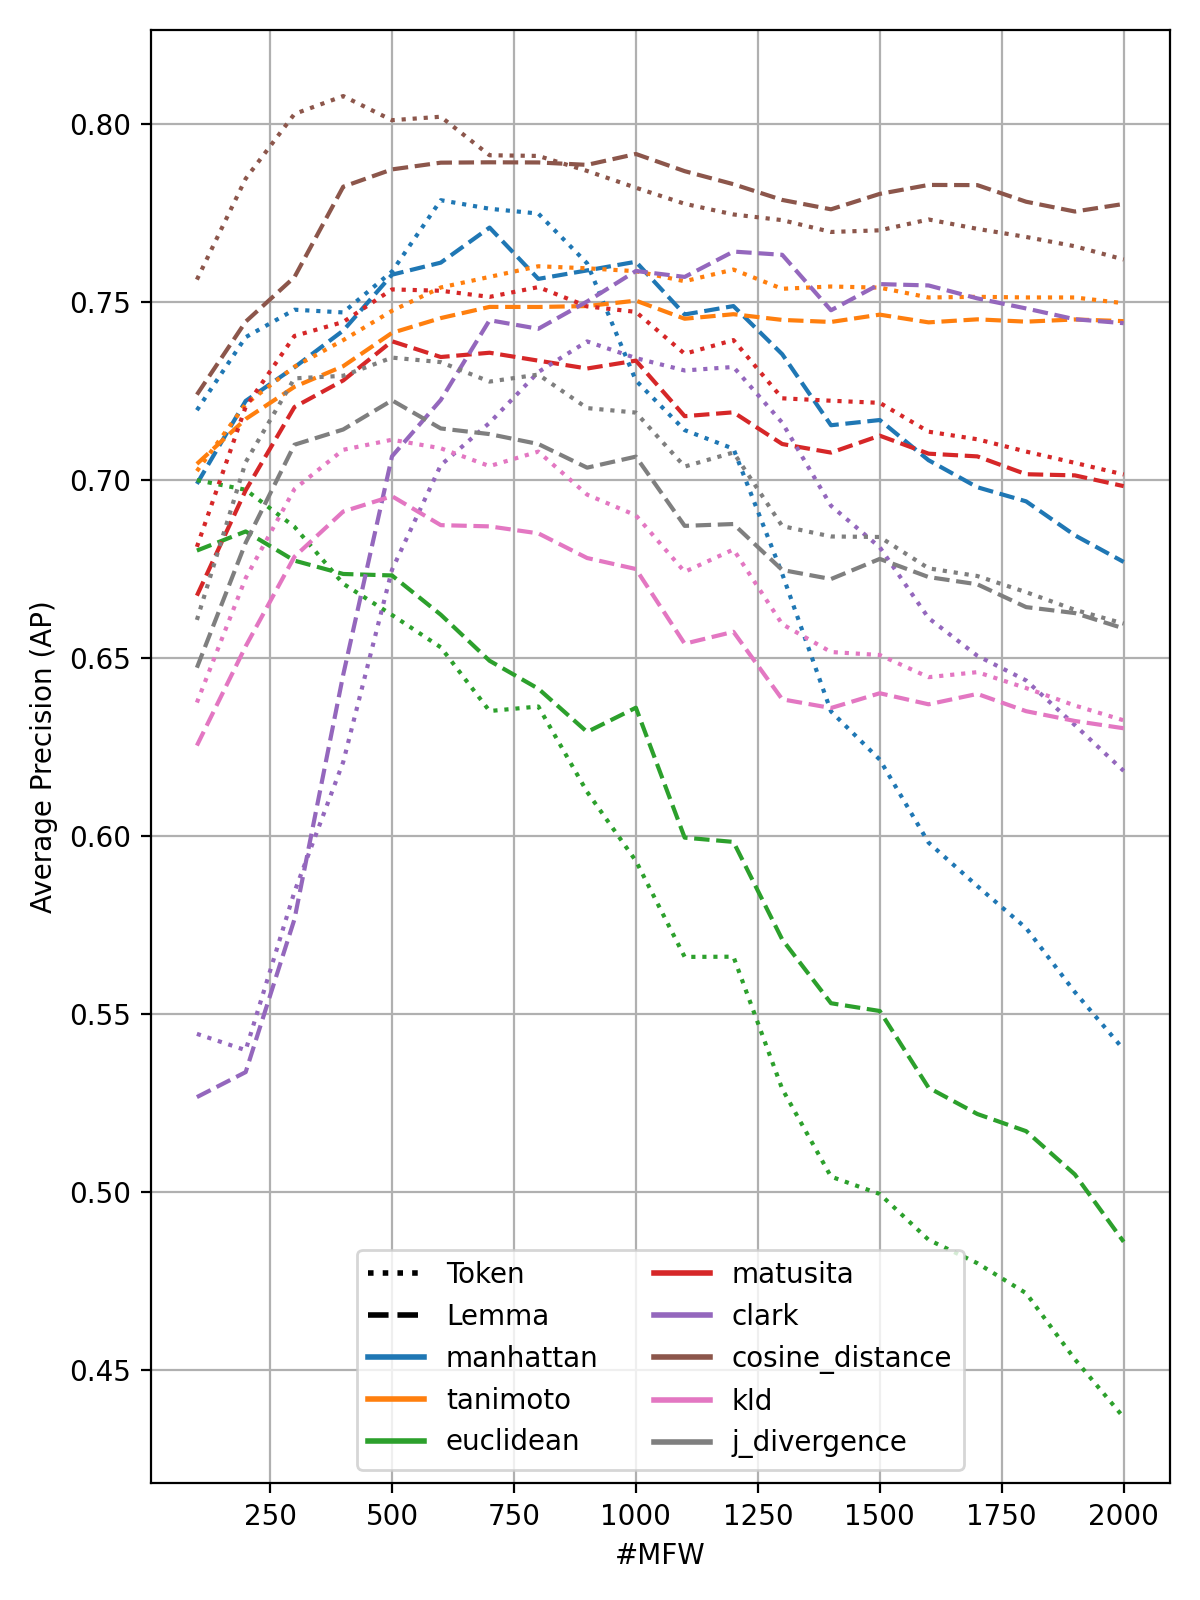
\includegraphics[width=0.9\linewidth]{img/token_vs_lemma_st_jean.png}
\end{figure}

\subsubsection{MFW Letter $n$-grams}

In this experiment the whole text is considered to create letter $n$-grams for the text representation, see Definition~\ref{def:letters_n_grams}.
As for the other experiment the MFW approach is used to create the feature vector.
On these vectors the distance measure used to create the rank list is the z-score normalized cosine distance.
The goal is to compare the influence of $n$ parameter of the $n$-grams over the size of the feature vector.
The parameters used are: a varying MFW vector size ranging between 500 and 15000 with a step of 500 and a $n$ for the following values : $3, 4, 5, (2, 3), (3, 4), (4, 5)$.
When considering letters $n$-grams the text representation increase size by a factor of approximately $t$, with $t$ being the average token length.
The number of different $n$-grams is not clear, but it is assumed to be larger than the vocabulary of the texts, thus the importance of having larger vector  when dealing with long texts such as the literature datasets.

Figure~\ref{fig:letter_ngrams} show the results of this experiment on the Oxquarry dataset (\ref{fig:letter_ngrams}) and Brunet dataset (\ref{fig:letter_ngrams_brunet}).

\begin{figure}
  \caption{Letters $n$-grams representation over number of MFW with different n}
  \label{fig:letter_ngrams}

  \subcaption{Oxquarry}
  \label{fig:letter_ngrams_oxquarry}
  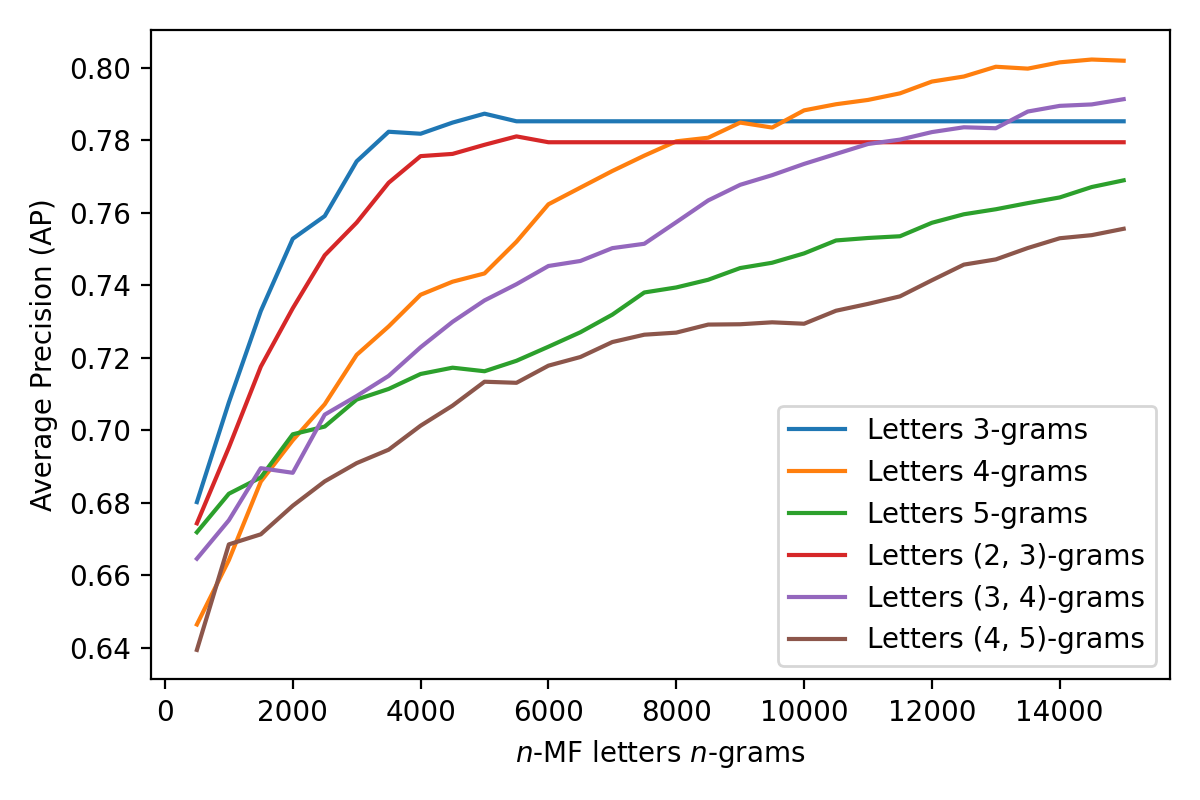
\includegraphics[width=\linewidth]{img/letter_ngrams_oxquarry.png}

  \subcaption{Brunet}
  \label{fig:letter_ngrams_brunet}
  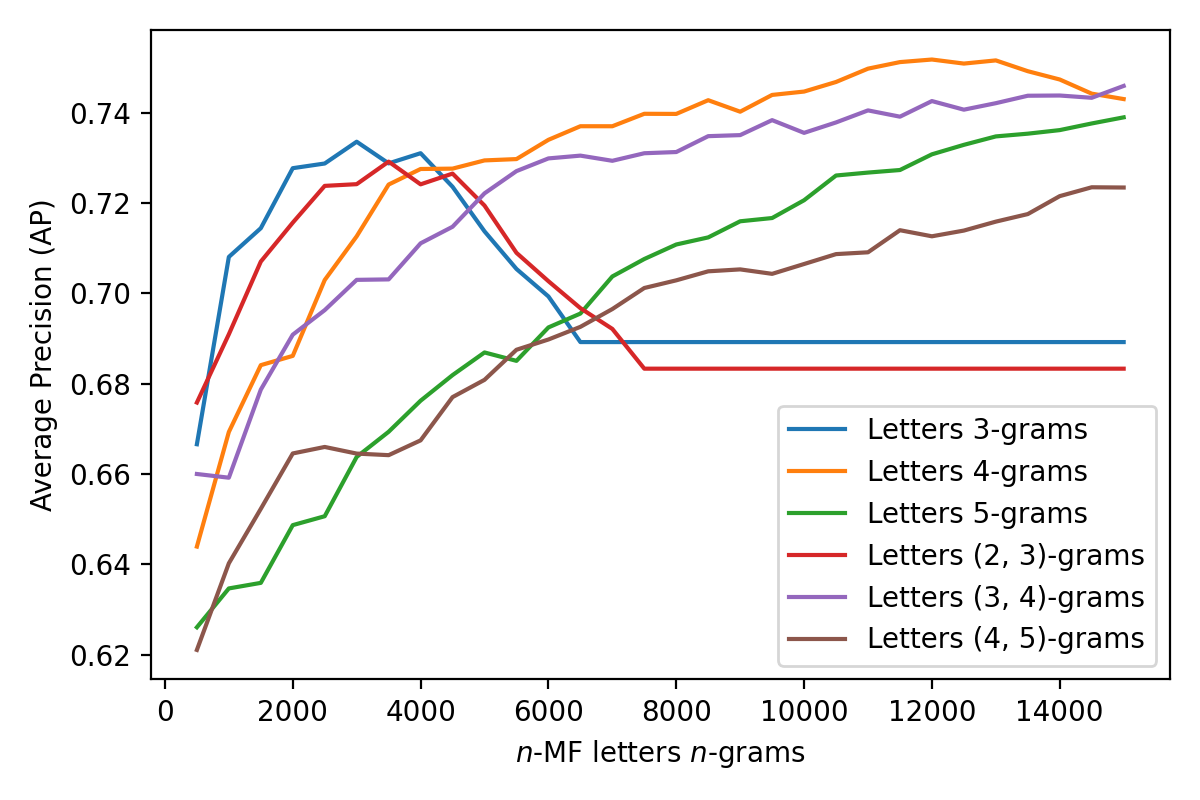
\includegraphics[width=\linewidth]{img/letter_ngrams_brunet.png}
\end{figure}


\subsubsection{MFW First letters, last letters, word n-grams of tokens}

In this experiment, the goal is to create 3 types of text representations of word substrings and compare them.

\begin{enumerate}
  \item
  The first representation is the N-first letter of each word tokens which correspond generaly to the meaning of a word.
  This approach is closely related to the lemma approach.
  \item
  Extract also the N-last letter of each word tokens which in this case correspond to the role of the word in a sentence.
  This second approach is closely related to the POS approach.
  \item
  The word $n$-grams (See Definition~\ref{def:words_n_grams}), this special type of n-grams only consider $n$-grams within a word.
  This exclude every overlapping word $n$-grams.
  This decision is made for this experiment such that interwords style information can't be learned and have a fair comparaison of these 3 texts representations.
\end{enumerate}
The two first methods can be considered as a subsample of the $n$-grams approach, thus a simplified one (have smaller text representation).
The distance measure used is the z-normalized cosine distance and the evaluation metric is the average precision.
The number of MFW variate for this experiment between 200 and 4000 with a step of 100.

Figure~\ref{fig:first_last_letters_ngrams_brunet} shows the results for the Brunet dataset and Figure~\ref{fig:first_last_letters_ngrams_oxquarry} for the oxquarry dataset.

In both dataset, the 3-last letters and 3-first letters gives a lower average precision and quickly converge to a equilibrium value at around 1500 MFW.
5-letters representations tend to produce better results than 3-letters and 4-letters representation as the MFW increase.
In the Oxquarry corpus, word 4-grams and word 5-grams give the better results with an average precision of ~95.0\%
For the brunet dataset, the 5-first letters can a good results compared to other text representations with small MFW vector size.

\begin{figure}
  \centering
  \caption{Average precision over the MFW in the rank list generated using the z-score normalized cosine distance}

  \subcaption{Oxquarry}
  \label{fig:first_last_letters_ngrams_oxquarry}
  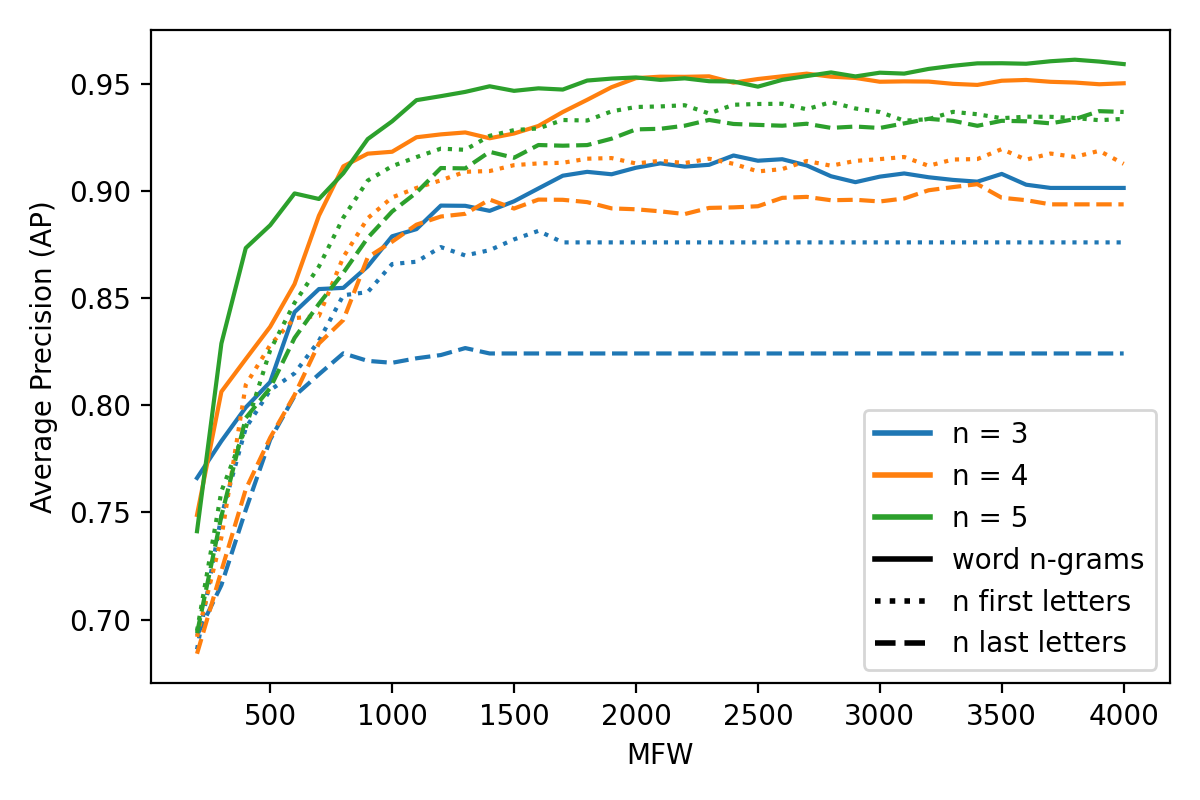
\includegraphics[width=\linewidth]{img/first_last_letters_ngrams_oxquarry.png}

  \subcaption{Brunet}
  \label{fig:first_last_letters_ngrams_brunet}
  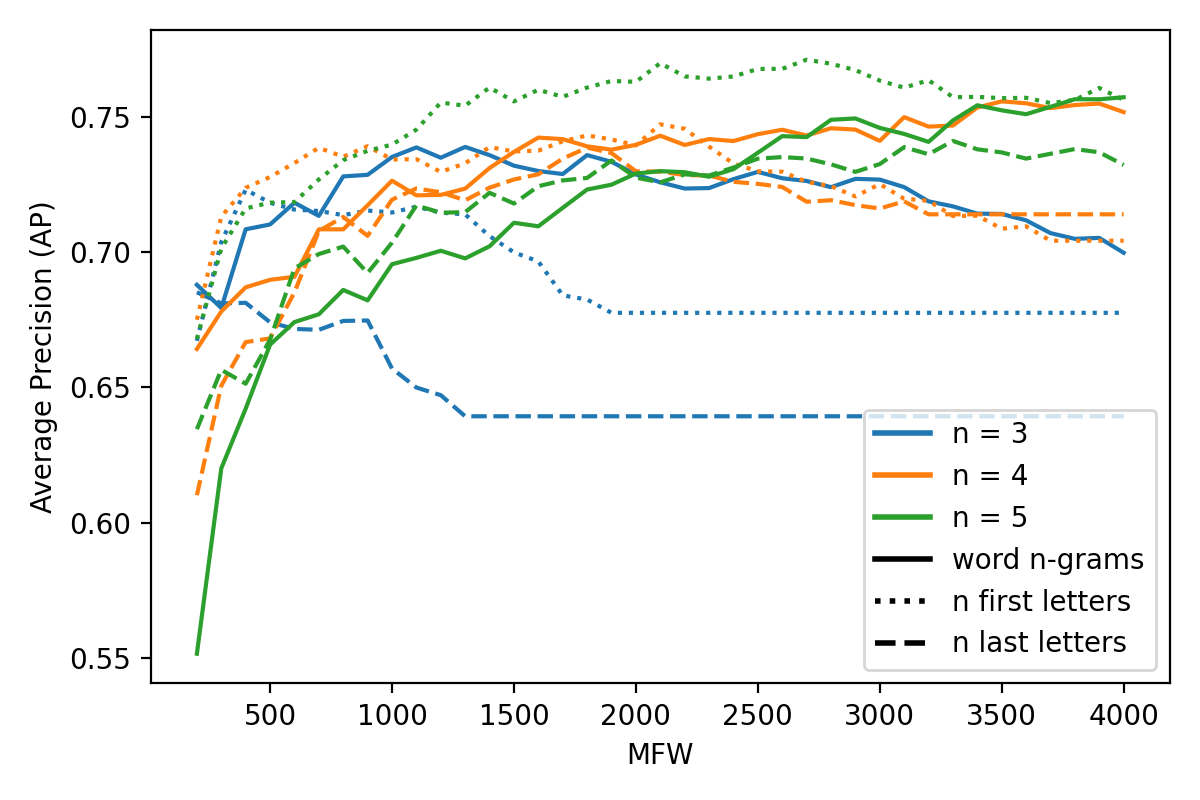
\includegraphics[width=\linewidth]{img/first_last_letters_ngrams_brunet.png}
\end{figure}

\subsubsection{MFW POS $n$-grams}

For this experiment short combination of POS are used to detect the style of the author.
The St-Jean dataset have for every word a POS tag, by using these POS tags and combining them using Definition~\ref{def:letters_n_grams} to create $n$-grams/w-shingling, a new text representation is obtained.
Using this representation the N-MFW are computed and the rank list containing every document pairs can be computed.

In this experiment, only 2-grams, 3-grams, 4-grams and the combination of the 2-grams and 3-grams denoted: (2, 3)-grams is used.
The distance metric used is the smoothed z-score normalized cosine distance.
For this representation no clear MFW (most frequent word, in this case POS $n$-grams are considered as words) vector size is advised, the size used is between 200 and 2000 with a step of 100.
Figure~\ref{fig:pos_ngrams} show the average precision on the rank list produced by using POS $n$-grams over the number of MFW.

The two following informations can be intuitively observed on this plot:
\begin{itemize}
  \item
  A more complex POS $n$-grams require more MFW to archive its maximal effectiveness.
  In the St-Jean corpus 26 POS are used to describe every words in the corpus.
  Which correspond to $26^2 = 676$ possible unique POS 2-grams, to $26^3 = 17'576$ POS 3-grams and $26^4 = 456'976$ POS 4-grams.
  \item
  Like other methods, if the MFW ceiling is too high, an overfitting to less important words is possible, thus reducing the average precision.
  In Figure~\ref{fig:pos_ngrams} the POS 2-grams clearly have a drop in average precision after \~250-MFW.
\end{itemize}

\begin{figure}
  \centering
  \caption{Average precision over the MFW in the rank list generated using the z-score normalized cosine distance.}
  \label{fig:pos_ngrams}
  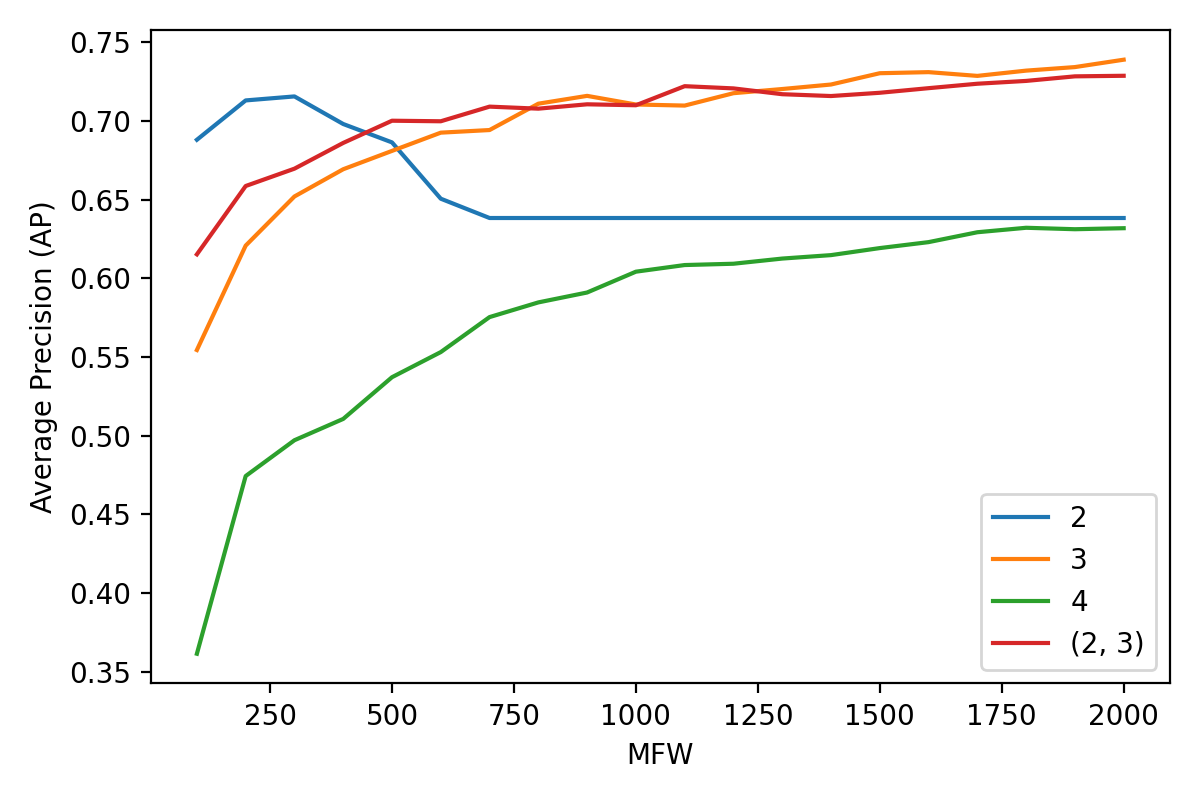
\includegraphics[width=\linewidth]{img/pos_ngrams.png}
\end{figure}

\subsubsection{Compression based distances}

This experiment try to compare the three proposed compression algorithm (GZip, BZip2, LZMA) for the compression based distance ranking.
For each algorithm for each document the size after compression is computed, as well as the concatenation of every document pairs.
Using these sizes and the NCD and CBC distance metrics (ref. Section~\ref{sec:compression_based_distances}, the rank list is evaluated.
This experiment is run on the three datasets three times to have a better approximation of the run time.
The results in terms of efficiency of the resulting rank list are shown in Table~\ref{tab:compression_evaluation}.
The average time of the 3 runs are in Table~\ref{tab:compression_evaluation_time}.

GZip seem to be giving the worse results on every dataset with an average AP of \~-0.20 in compared to LZMA and BZip2.
LZMA give the best results on every dataset tested, but BZip2 have close results.
The cosine-based compression distance (CBC) tend to give better results over the normalized compression distance (NCD).
In terms of time complexity BZip2 is the fastest algorithm of the 3 proposed, LZMA is ~5-6 times slower than BZip2, and GZip slower than BZip2 by around ~5-20\%.
No significant time differences is recorded between the NCD and CBC distance measures, since the greater complexity is in the compression algorithm.

% \begin{figure}
%   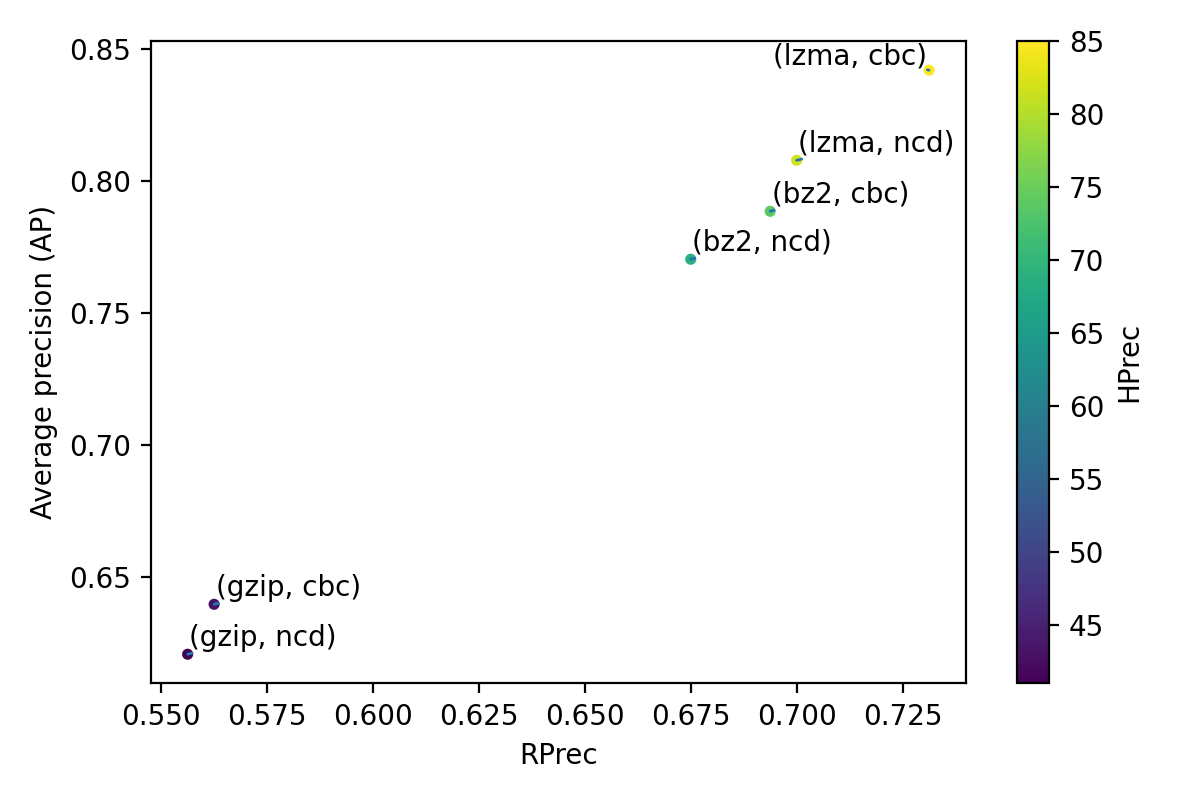
\includegraphics[width=\linewidth]{img/compression_evaluation_oxquarry.png}
%   \caption{Evaluation of the different compression algorithm and distance metrics on Oxquarry}
%   \label{fig:compression_evaluation_oxquarry}
% \end{figure}

\begin{table}
  \centering
  \caption{Evaluation of the different compression algorithm and distance metrics using Average Precision (AP), R-Precision (RP) and High Precision (HP)}
  \label{tab:compression_evaluation}

  \subcaption{Oxquarry}
  \label{tab:compression_evaluation_oxquarry}
  \begin{tabular}{l c c}
    \toprule
    AP/RPrec/HPrec & NCD          & CBC \\
    \midrule
    Bzip2          & 0.77/0.68/69 & 0.79/0.69/74 \\
    GZip           & 0.62/0.56/41 & 0.64/0.56/43 \\
    LZMA           & 0.81/0.70/82 & 0.84/0.73/85 \\
    \bottomrule
  \end{tabular}

  \subcaption{Brunet}
  \label{tab:compression_evaluation_brunet}
  \begin{tabular}{l c c}
    \toprule
    AP/RPrec/HPrec & NCD          & CBC \\
    \midrule
    Bzip2          & 0.76/0.70/25 & 0.76/0.70/25 \\
    GZip           & 0.61/0.53/24 & 0.60/0.52/23 \\
    LZMA           & 0.78/0.73/27 & 0.79/0.73/31 \\
    \bottomrule
  \end{tabular}

  \subcaption{St-Jean}
  \label{tab:compression_evaluation_st_jean}
  \begin{tabular}{l c c}
    \toprule
    AP/RPrec/HPrec & NCD           & CBC \\
    \midrule
    Bzip2          & 0.70/0.63/214 & 0.70/0.62/219 \\
    GZip           & 0.45/0.44/54  & 0.42/0.42/56 \\
    LZMA           & 0.71/0.63/241 & 0.71/0.62/214 \\
    \bottomrule
  \end{tabular}
\end{table}

\begin{table}
  \centering
  \label{tab:compression_evaluation_time}
  \caption{Average run time for the rank list computation with the different compression algorithm and distance metrics}

  \subcaption{Oxquarry}
  \label{tab:compression_evaluation_time_oxquarry}
  \begin{tabular}{l c c}
    \toprule
    Time      & NCD   & CBC \\
    \midrule
    Bzip2     & 12.7s & 12.7s \\
    GZip      & 15.0s & 14.9s \\
    LZMA      & 69.0s & 68.8s \\
    \bottomrule
  \end{tabular}

  \subcaption{Brunet}
  \label{tab:compression_evaluation_time_brunet}
  \begin{tabular}{l c c}
    \toprule
    Time      & NCD   & CBC \\
    \midrule
    Bzip2     & 8.4s & 8.4s \\
    GZip      & 8.8s & 8.9s \\
    LZMA      & 46.6s & 46.8s \\
    \bottomrule
  \end{tabular}

  \subcaption{St-Jean}
  \label{tab:compression_evaluation_time_st_jean}
  \begin{tabular}{l c c}
    \toprule
    Time      & NCD    & CBC \\
    \midrule
    Bzip2     & 198.9s  & 198.4s \\
    GZip      & 211.3s  & 214.5s \\
    LZMA      & 1046.3s & 1052.0s \\
    \bottomrule
  \end{tabular}
\end{table}


\subsubsection{Frequent errors}
\label{sec:frequent_errors}

This section try to understand the errors in our system, in this case the false links (document pairs with different authors) highly ranked on different rank list.
The rank list quality is highly based on the feature vector created using the N-MFW, having a good understanding of this vector give good indications of the strength of the system.

To find recurrent errors in our system we use 5 different distance metrics (Manhattan, Tanimoto, Clark, Matusita, Cosine distance) on the relative frequency of the 500-MFW using the St-Jean dataset.
This generates 5 rank lists.
The average precision for these rank list is always greater than 0.7.
With this 5 rank lists only the top 10 false links are kept to be analyzed.
Frequent errors are links that often appear in this top 10.
Figures~\ref{fig:mfw_vector_error} show two pairs (Zola 49 / Flaubert 63 and Maupassant 10 / Flaubert 52) that appear 4 time out of the 5 rank lists in the top 10 false links, thus frequent error.

\begin{figure}
  \centering
  \caption{Example of 500-MFW relative frequency vectors for the two documents in a reccurant (4 rank lists out of 5) false link in the top 10 false links}
  \label{fig:mfw_vector_error}

  \subcaption{First example}
  \label{fig:mfw_vector_error_0}
  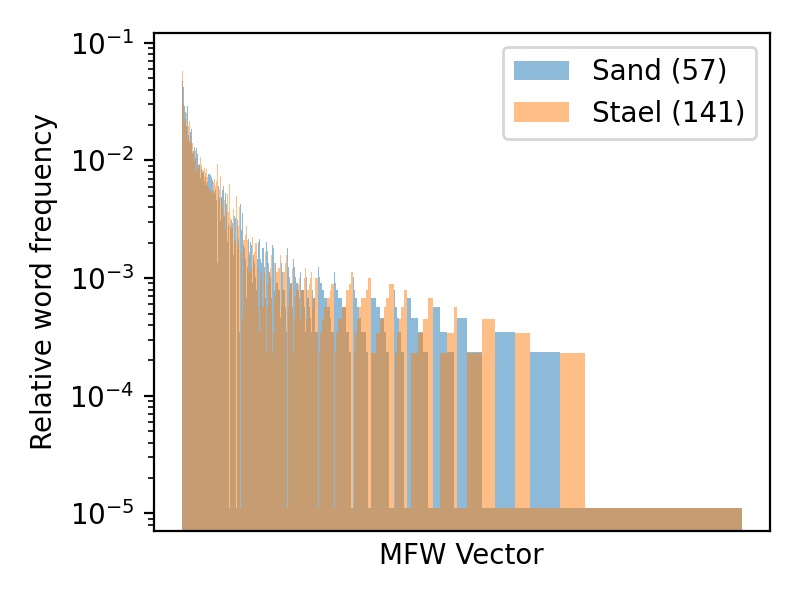
\includegraphics[width=\linewidth]{img/mfw_vector_error_0.png}

  \subcaption{Second example}
  \label{fig:mfw_vector_error_1}
  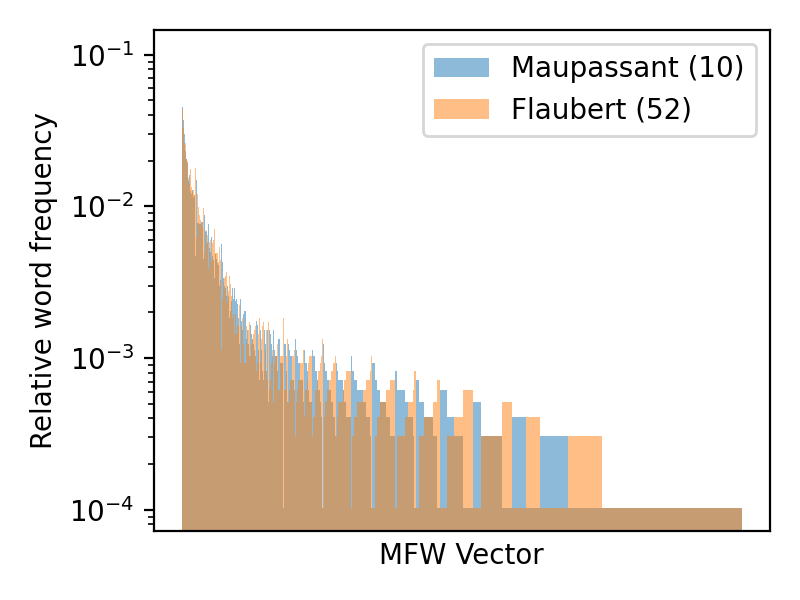
\includegraphics[width=\linewidth]{img/mfw_vector_error_1.png}
\end{figure}

To be able to understand more easily this vector, the values have been sorted by relative frequencies and using the logarithmic scale.
When a large proportion of the vectors overlap it indicates a high similarity between the MFW vectors.
In this case most of the surface overlap, so the distance function will give a low value, and rank this vector high in the list.
Both document style are close when their feature vector are closely related.
We can not clearly determinate that these texts are from a different author using only this type of representation.
These two vectors pair can be visually compared to the most similar link (ranked 1 using Manhattan distance) in Figure~\ref{fig:mfw_vector_first_rl} (Stael 157 / Steal 183) or the HPrec-th (last continous correct pair from the top of the list) in Figure~\ref{fig:mfw_vector_first_last_rl} (Maupassant 10 / Maupassant 67), both of these links show a large proportion of overlapping surface.
A counter example would be the least similar link (ranked last using Manhattan distance) which represent a negatively correlated document pair, Figure~\ref{fig:mfw_vector_last_rl} showcase this link.
As expected, most of this figure surface is non-overlapping.

\begin{figure}
  \centering
  \caption{500-MFW relative frequency for the two documents ranked $X$ in the rank list}

  \subcaption{$X$ = First}
  \label{fig:mfw_vector_first_rl}
  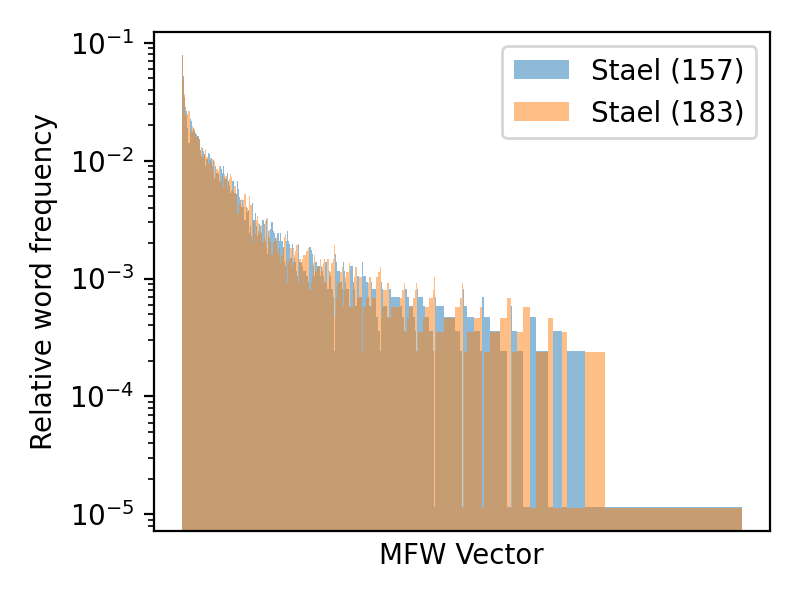
\includegraphics[width=\linewidth]{img/mfw_vector_first_rl.png}

  \subcaption{$X$ = HPrec-th}
  \label{fig:mfw_vector_first_last_rl}
  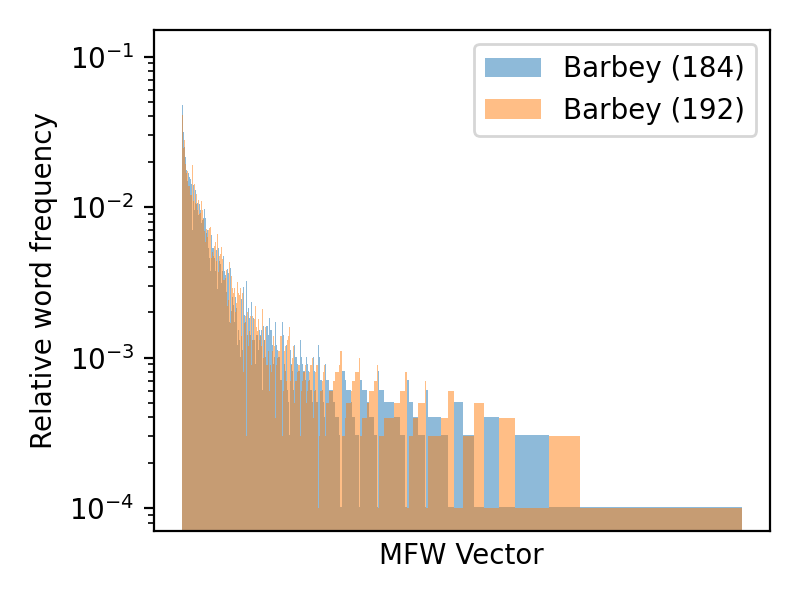
\includegraphics[width=\linewidth]{img/mfw_vector_first_last_rl.png}

  \subcaption{$X$ = Last}
  \label{fig:mfw_vector_last_rl}
  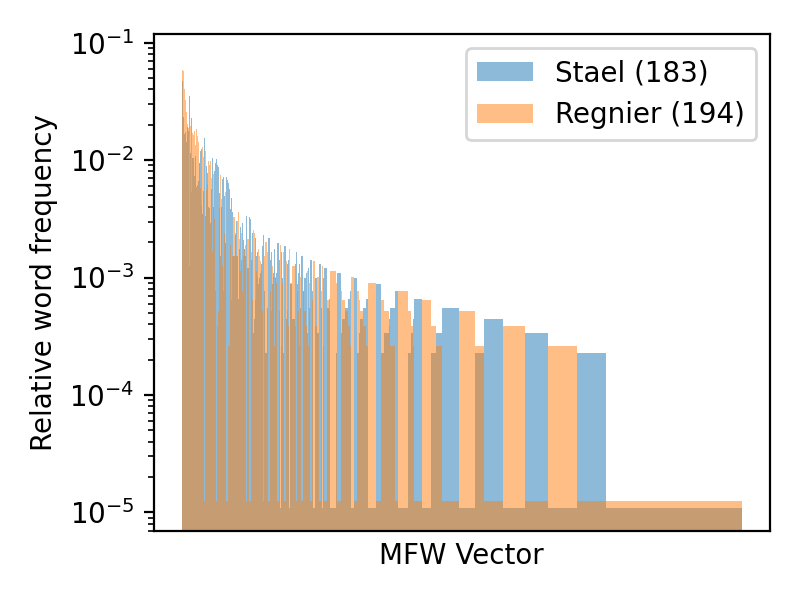
\includegraphics[width=\linewidth]{img/mfw_vector_last_rl.png}
\end{figure}

\subsubsection{Publication date differences analyis}

When dealing with false links ranked high in the rank list, as the previous experiment showed, some excerpt use similar words.
These shared words might be related to the era the book was written in.
The following experiment try to investigate on this.

In the St-Jean dataset publication paper, the publication dates of each excepts are available~\cite{st_jean}.
First the publication date distribution of the dataset must be understood.
Figure~\ref{fig:dates_distribution} show the distribution of the publication date in the St-Jean dataset.
The date difference distribution for each pair of documents can be computed, Figure~\ref{fig:dates_differences_all} show case this.
We can see that the average date difference in the dataset is 28.24 years with a standard deviation of 20.73 years.
Since this dataset contain multiple excerpt from the same book, we might consider only the links of different authors (false links).
Figure~\ref{fig:dates_differences_false} shows the date differrence distribution of the false links.
As expected the mean increased to 29.04 years since there are fewer links with small date difference.
Same authors links (true links) are displayed in Figure~\ref{fig:dates_differences_r_true}, they confirm the previous statement that most of the same authors links have a low date difference with a mean of 5.11 years.

\begin{figure}
  \centering
  \caption{Dates and Date differences denstiy distributions on St-Jean for every excerpt}

  \subcaption{Date distribution}
  \label{fig:dates_distribution}
  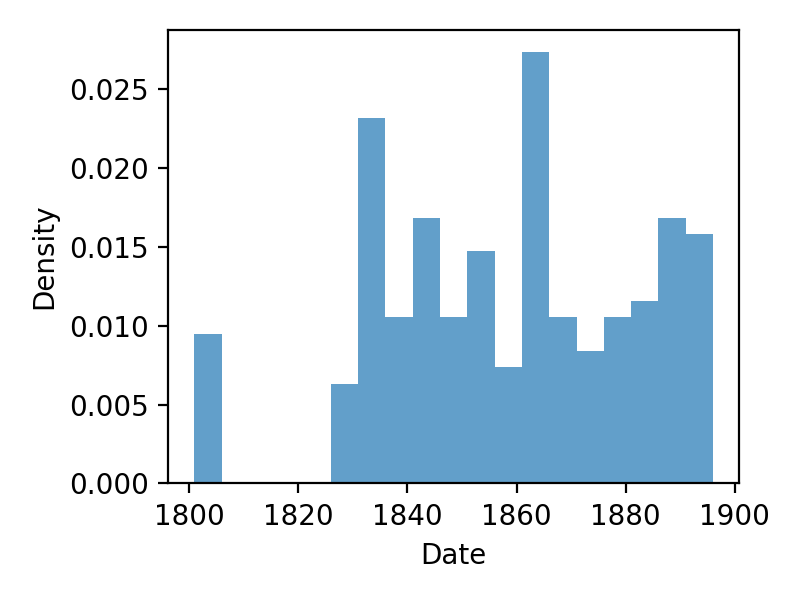
\includegraphics[width=\linewidth]{img/dates_distribution.png}

  \subcaption{Date difference denstiy distributions}
  \label{fig:dates_differences_all}
  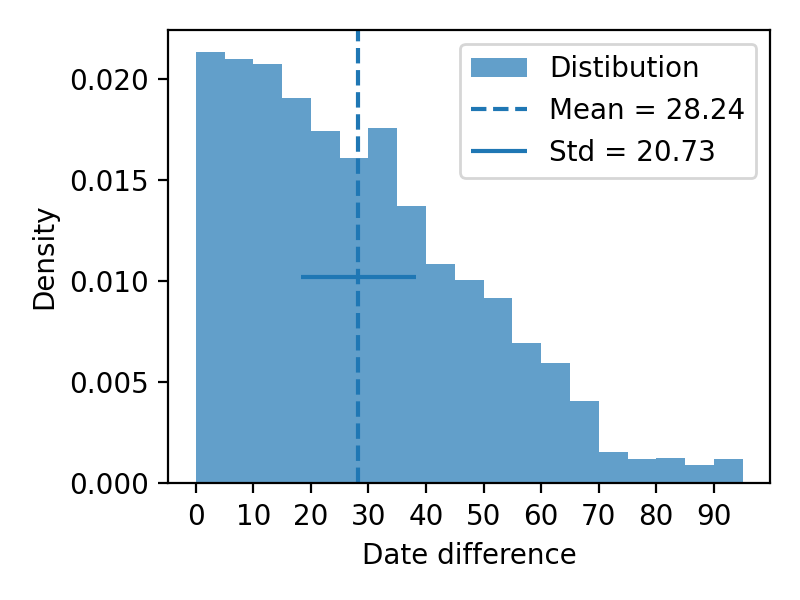
\includegraphics[width=\linewidth]{img/dates_differences_all.png}
\end{figure}

\begin{figure}
  \centering
  \caption{Date difference denstiy distributions in St-Jean}

  \subcaption{False links}
  \label{fig:dates_differences_false}
  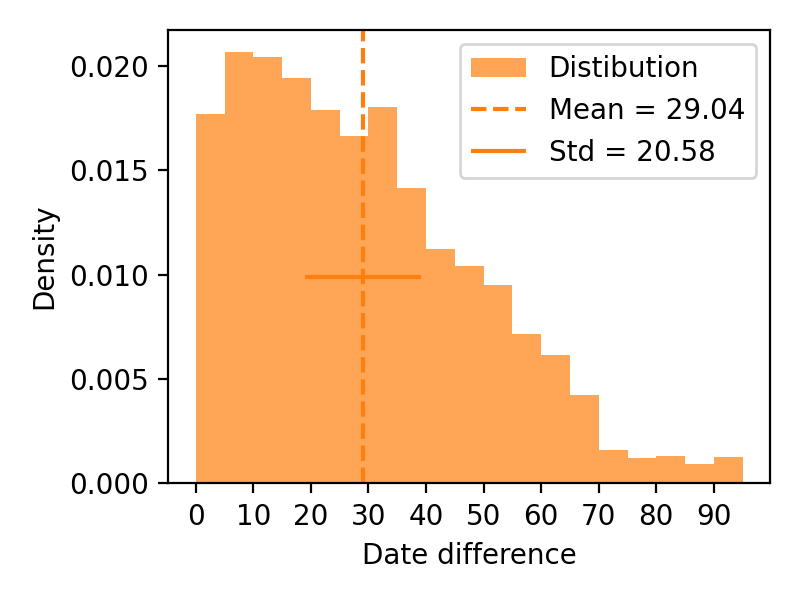
\includegraphics[width=\linewidth]{img/dates_differences_false.png}

  \subcaption{True links}
  \label{fig:dates_differences_r_true}
  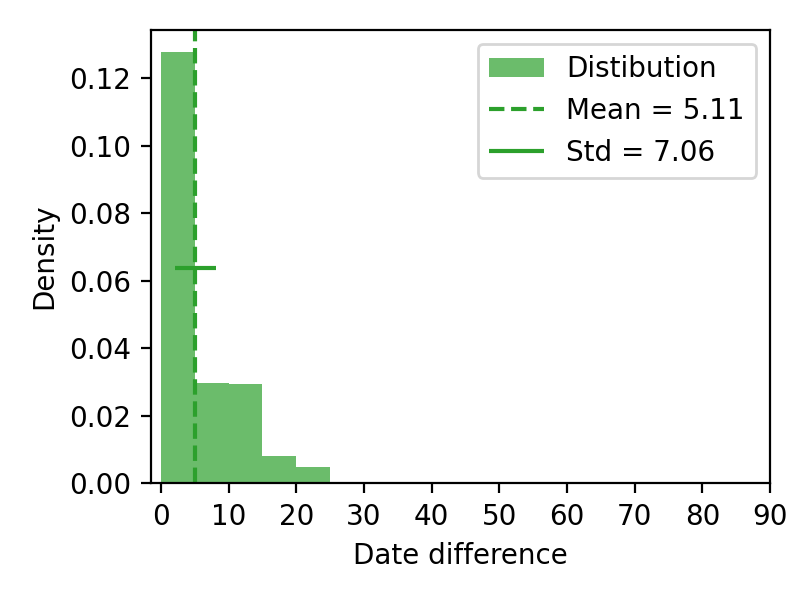
\includegraphics[width=\linewidth]{img/dates_differences_r_true.png}

  \subcaption{Top-r false links using a rank list with 80\% average precision.}
  \label{fig:dates_differences_r_false}
  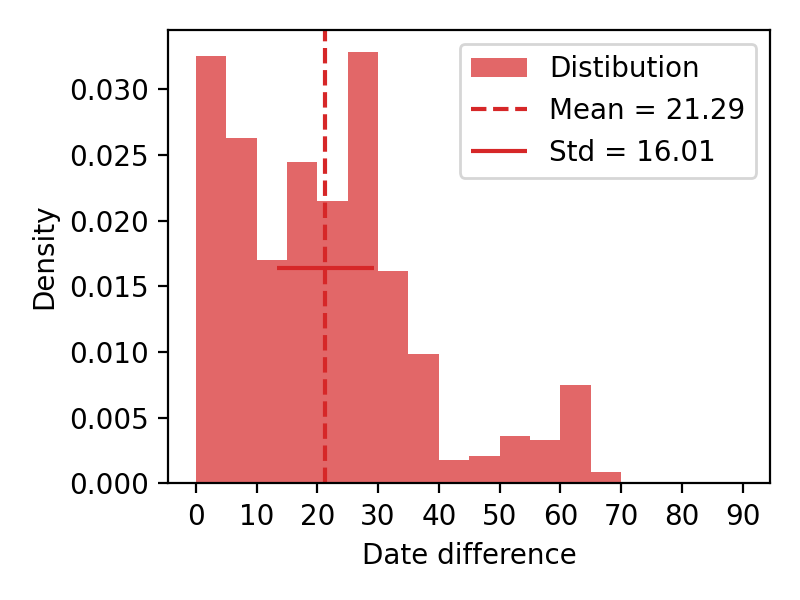
\includegraphics[width=\linewidth]{img/dates_differences_r_false.png}
\end{figure}

Figure~\ref{fig:dates_differences_r_false} show the date difference density on the top-r false links (670 in case of St-Jean) on a rank list with 80\% average precision (obtained by fusing the 5 ranks list used and presented in frequent error, ref. Section~\ref{sec:rank_list_fusion}~and~\ref{sec:frequent_errors}).
Two interesting information can be extracted here.
First the mean is lower by 8.22 years (29.04 - 20.82) comparing to the false links distribution which clearly indicate the importance of publication date in the ranking of the documents.
Secondly we can observe a drop after 35 years of date difference, which indicate that links in the interval $\left[0-35\right]$ years are harder to discriminate between a true link and a false link than links outside this interval.
This 35 years interval can be related to the generation factor, the age of woman giving birth is around 25-34 in France~\cite{generations}, the birth country of the authors in this dataset.
Each new generation tend to use its own vocabulary, and thus it can be harder to discriminate author of text belonging to the same generation, in the other hand having different vocabulary can indicate a different time period and is often used to detect document forgery~\cite{savoy_stylo}.

\subsubsection{Rank lists fusion evaluation}

In this experiment, the goal to understand if fusing rank list can improve performance of the rank list.
The methodology used, is to create multiple rank lists and fuse them for every 4 rank lists combinations.

The rank used are the ones obtained by using the following distances' metrics : Manhattan, Tanimoto, Clark, Matusita, Cosine Distance, Kullback-Leibler divergence on both the top 500 MFW tokens and the top 750 MFW tokens 3-grams, with smoothing for all of them.
This creates 12 rank lists, every 4 combinations of these 12 rank lists creates 495 possible fusions ($C^{12}_{4} = 495$).
For this 495 fusions, the 3 metrics: Average Precision (AP), R-Precision (RPrec) and High Precision (HPrec).
The results are graphically presented in Figure~\ref{fig:fusions} for the dataset Oxquarry~(\ref{fig:fusion_oxquarry}), Brunet~(\ref{fig:fusion_brunet}) and St-Jean~(\ref{fig:fusion_st_jean}).

\begin{figure}
  \centering
  \caption{Evaluation of every combination of 4 rank list fusions using Z-Score and S-Curve}
  \label{fig:fusions}

  \subcaption{Oxquarry}
  \label{fig:fusion_oxquarry}
  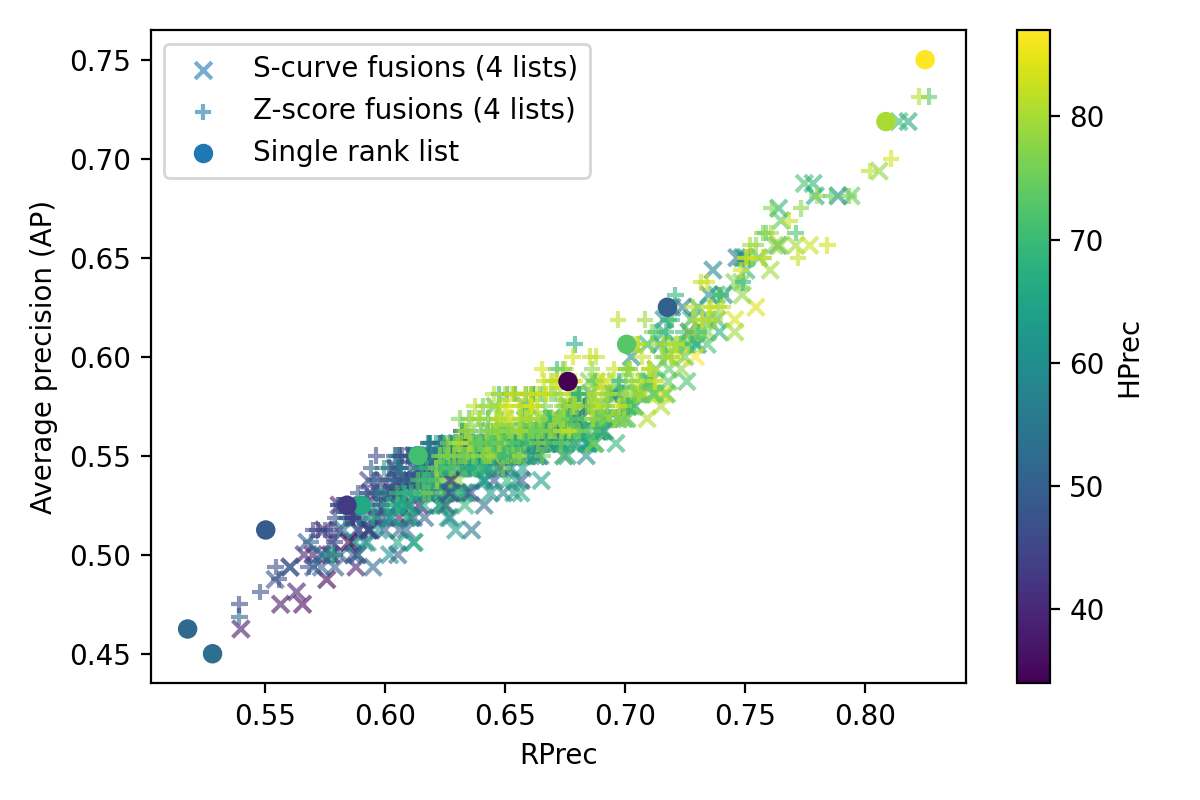
\includegraphics[width=\linewidth]{img/fusion_oxquarry.png}

  \subcaption{Brunet}
  \label{fig:fusion_brunet}
  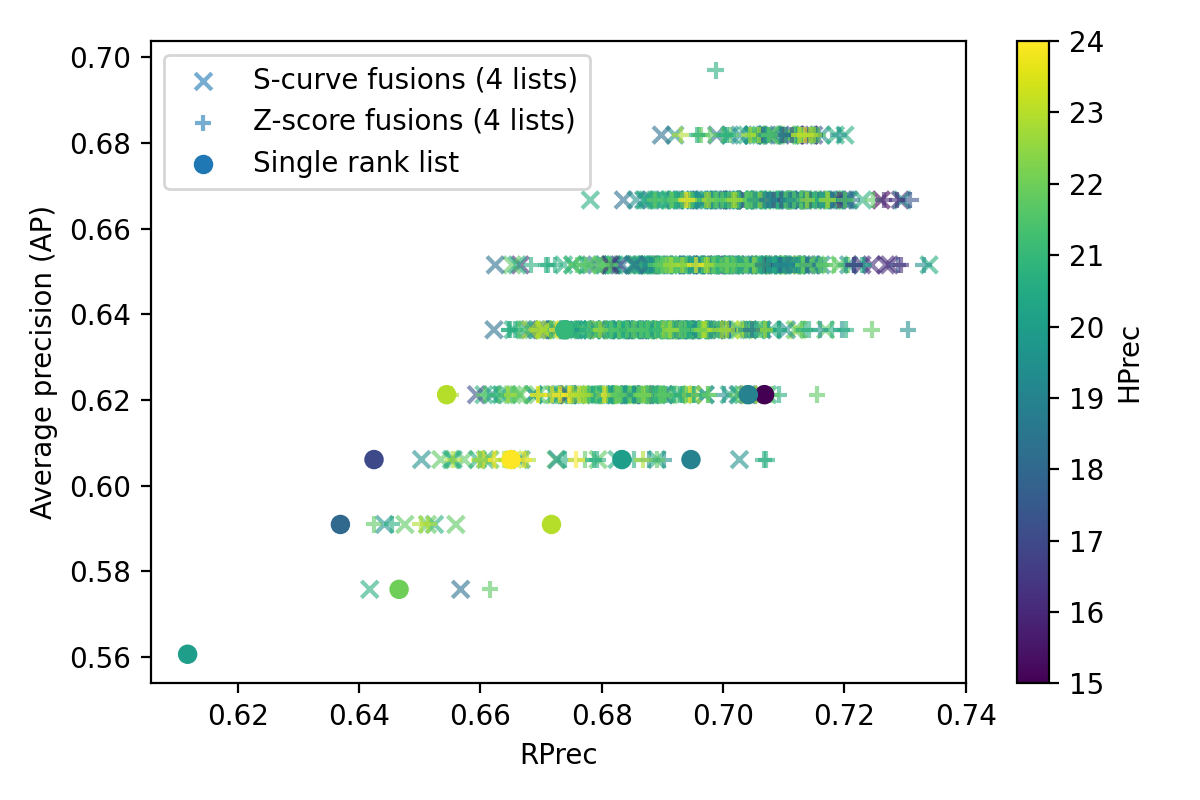
\includegraphics[width=\linewidth]{img/fusion_brunet.png}

  \subcaption{St-Jean}
  \label{fig:fusion_st_jean}
  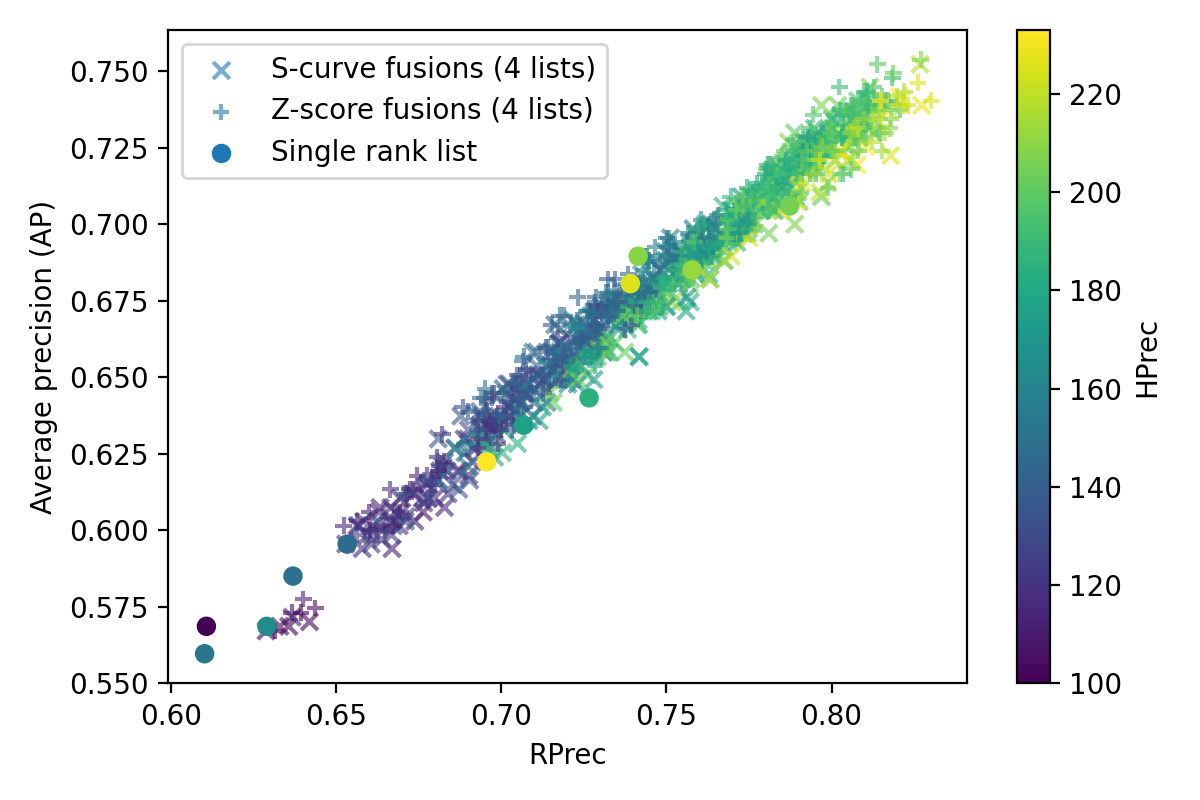
\includegraphics[width=\linewidth]{img/fusion_st_jean.png}
\end{figure}

To compare the rank list produced by both the S-Curve and Z-Score fusions to the non-fused rank list, the best metrics of each rank list used for each fusion (denoted \textit{Single-Max}) is compared using a sign test to the rank list produced by S-Curve fusion in Table~\ref{tab:s_curve_single_max}.
The Single-Max comparison to the Z-Score fusion in Table~\ref{tab:z_score_single_max} and a comparison Z-Score / S-Curve fusion in Table~\ref{tab:s_curve_z_score}.

\begin{table*}
  \centering
  \caption{Rank list sign test, * : Binomial test p-value < 5\%}
  \label{tab:fusion_sign_test_comparaisons}

  \subcaption{S-Curve/Equal/Single max}
  \label{tab:s_curve_single_max}
  \begin{tabular}{l c c c c}
    \toprule
    Metric         & St-Jean     & Brunet      & Oxquarry    & \textbf{Total} \\ \midrule
    AP             & 161/0/334*  & 208/0/287*  & 1/0/494*    & 370/0/1115*    \\
    RPrec          & 169/9/317*  & *378/75/42  & 0/2/493*    & 547/86/852*    \\
    HPrec          & *287/1/207  & 49/87/359*  & 32/11/452*  & 368/99/1018*   \\
    \textbf{Total} & 617/10/858* & 635/162/688 & 33/13/1439* & 1285/185/2985* \\
    \bottomrule
  \end{tabular}

  \subcaption{Z-Score/Equal/Single max}
  \label{tab:z_score_single_max}
  \begin{tabular}{l c c c c}
    \toprule
    Metric        & St-Jean     & Brunet      & Oxquarry    & \textbf{Total} \\ \midrule
    AP            & *284/0/211  & *285/0/210  & 1/0/494*    & 570/0/915*     \\
    RPrec         & *312/10/173 & *361/94/40  & 0/0/495*    & 673/104/708    \\
    HPrec         & *289/0/206  & 35/63/397*  & 79/13/403*  & 403/76/1006*   \\
    \textbf{Total}& *885/10/590 & 681/157/647 & 80/13/1392* & 1646/180/2629* \\
    \bottomrule
  \end{tabular}

  \subcaption{S-Curve/Equal/Z-Score}
  \label{tab:s_curve_z_score}
  \begin{tabular}{l c c c c}
    \toprule
    Metric        & St-Jean     & Brunet       & Oxquarry     & \textbf{Total} \\ \midrule
    AP            & 7/0/488*    & 42/0/453*    & *270/0/225   & 319/0/1166*    \\
    RPrec         & 4/3/488*    & 124/241/130  & 51/96/348*   & 179/340/966*   \\
    HPrec         & 57/18/420*  & *188/202/105 & 70/34/391*   & 315/254/916*   \\
    \textbf{Total}& 68/21/1396* & 354/443/688* & 391/130/964* & 813/594/3048*  \\
    \bottomrule
  \end{tabular}
\end{table*}

Using these distance metric on these datasets, the sign test tends to indicate that the fusion reduce the overall quality of the rank list compared to the best rank list in fusion.

But multiple points can be observed:
\begin{itemize}
  \item
  The three evaluations metrics are high correlated (especially Average Precision and R-Precision), the columns and lines \textit{Total} in the tables are to be lightly considered and not as an absolute proof.
  \item
  The Oxquarry dataset seem particularly not fitted for the fusion using the proposed distance metrics.
  This can be further explain by taking a look at the Figure~\ref{fig:fusion_oxquarry}.
  Most of the Single rank list in this dataset obtain average to poor results, except for two rank list with excellent results.
  Which considering the setup of the experiment, fusing a very good rank list with multiple bad rank list will certainly produce a rank list with worse results than the first one.
  The Oxquarry dataset may be an outlier in this experiment.
  \item
  On the St-Jean and Brunet dataset most of the metrics in the experiment Single Max vs Z-Score fusion (Table~\ref{tab:z_score_single_max}) produce significant results in favor of the fusion.
  \item
  The Z-score fusion seem to be giving better results on most metrics and datasets over the S-curve fusion.
  \item
  The HPrec is most of the time deteriorated with the fusion.
\end{itemize}

\subsection{Clustering}

\subsubsection{Clustering evaluation metrics}

To evaluate clustering, the metrics used are the BCubed~\cite{bcubed} family.
BCubed has shown to satisfy 4 importants constraints when evaluating clusterings : \textit{Cluster Homogeneity} (different categories should be in the different clusters), \textit{Cluster Completness} (same categories should belong to the same cluster) and the \textit{Rag Bag constraint} (noisy/miscellaneous categories should be in the same cluster and not in 'healthy' clusters) and the \textit{Cluster size vs quantity constraints} (favorise large cluster)~\cite{bcubed}.
These metrics are used in the clustering task at PAN@CLEF~\cite{pan16}.

\begin{definition}[Correctness~\cite{bcubed}]
  Let L(e) and C(e) be the category and the cluster of an element e.
  The correctness is following the biconditional condition on the category and cluster equality (biconditional: $A \Longleftrightarrow B \equiv (A \land B) \lor (\neg A \land \neg B)$).
  \begin{gather*}
    Correctness(e, e') = \\
    \begin{cases}
      1, & if (L(e) = L(e')) \Longleftrightarrow (C(e) = C(e'))\\
      0, & otherwise
    \end{cases}
  \end{gather*}
  In other terms, the correctness has a value of one if the two elements are in the both in the same cluster and has the same category OR both in a different cluster and a different category.
\end{definition}

\begin{definition}[$BCubed$ Precision~\cite{bcubed}]
  The $BCubed$ Precision correspond to the average of correctness for all elements on the average of all element such that \textbf{their cluster are the same}.
  \begin{equation}
    BCubed_{precision} = \text{Avg}_{e}[\text{Avg}_{e' C(e)=C(e')}[Correctness(e, e')]]
  \end{equation}
\end{definition}

\begin{definition}[$BCubed$ Recall~\cite{bcubed}]
  The $BCubed$ Recall correspond to the average of correctness for all elements on the average of all element such that \textbf{their category are the same}.
  \begin{equation}
    BCubed_{recall} = \text{Avg}_{e}[\text{Avg}_{e' L(e)=L(e')}[Correctness(e, e')]]
  \end{equation}
\end{definition}

\begin{definition}[$BCubed F_1$ Score~\cite{bcubed}]
  $BCubed F_1$ Score uses the harmonic mean between the $BCubed_{precision}$ and $BCubed_{recall}$.
  \begin{equation}
    BCubed_{F_1} =
    2 \cdot \frac{BCubed_{precision} \cdot BCubed_{recall}}
    {BCubed_{precision} + BCubed_{recall}}
  \end{equation}
  The $F_\beta$ measures provide a parametric way to represent with a single value the two counterbalancing measures in this case, the $BCubed F_1$ use the Precision and Recall $BCubed$, with the $F$ measures with $\beta = 1$.
\end{definition}

\subsubsection{Clustering unsupervised cut method}



\begin{figure}
  \caption{Unsupervised clustering on Oxquarry and Brunet}
  \label{fig:unsupervised_clustering_ob}

  \subcaption{Oxquarry}
  \label{fig:unsupervised_clustering_oxquarry}
  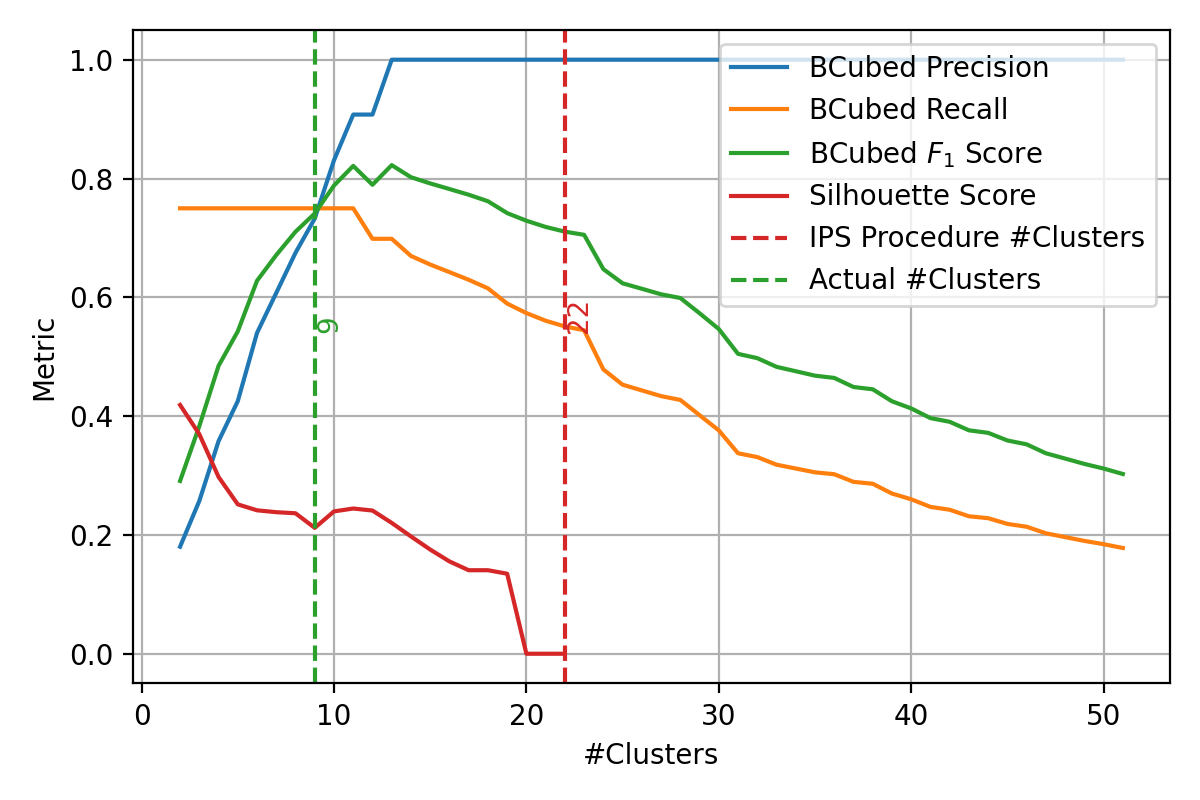
\includegraphics[width=\linewidth]{img/unsupervised_clustering_oxquarry.png}

  \subcaption{Brunet}
  \label{fig:unsupervised_clustering_brunet}
  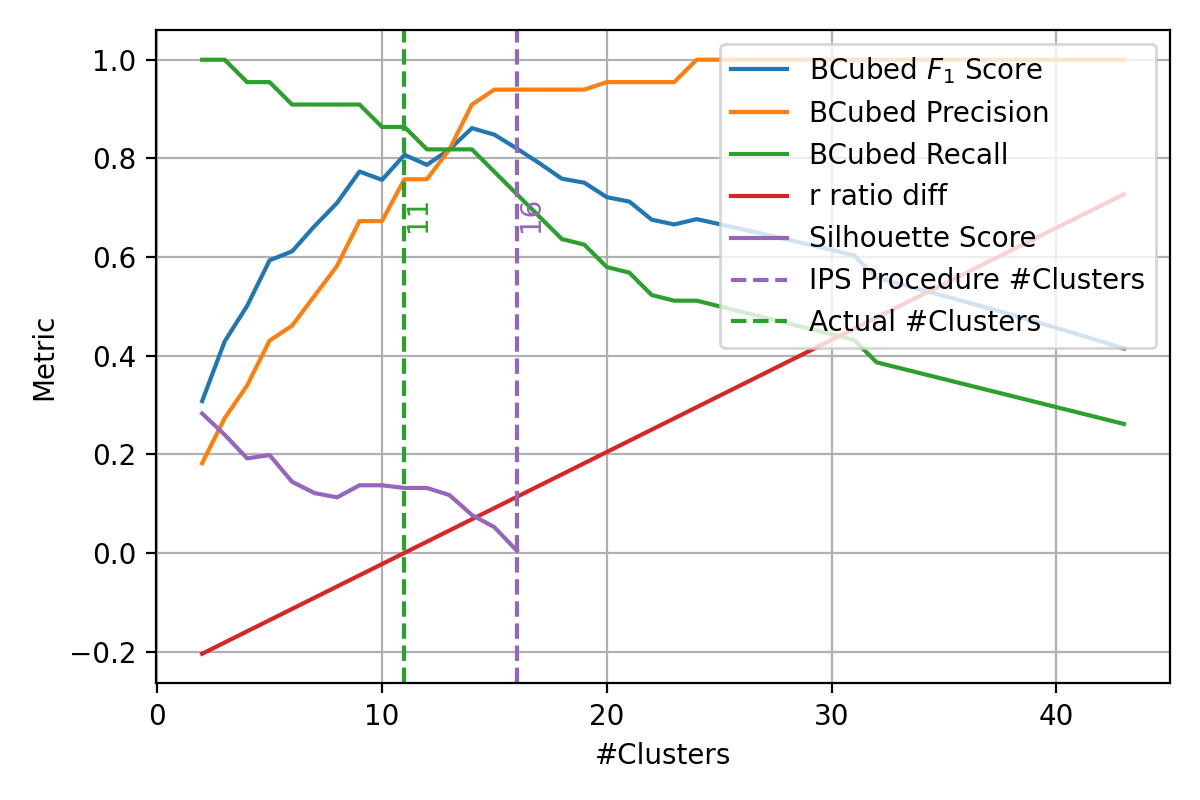
\includegraphics[width=\linewidth]{img/unsupervised_clustering_brunet.png}
\end{figure}

\begin{figure}
  \caption{Unsupervised clustering on St-Jean}
  \label{fig:unsupervised_clustering_sj}

  \subcaption{St-Jean A}
  \label{fig:unsupervised_clustering_st_jean_A}
  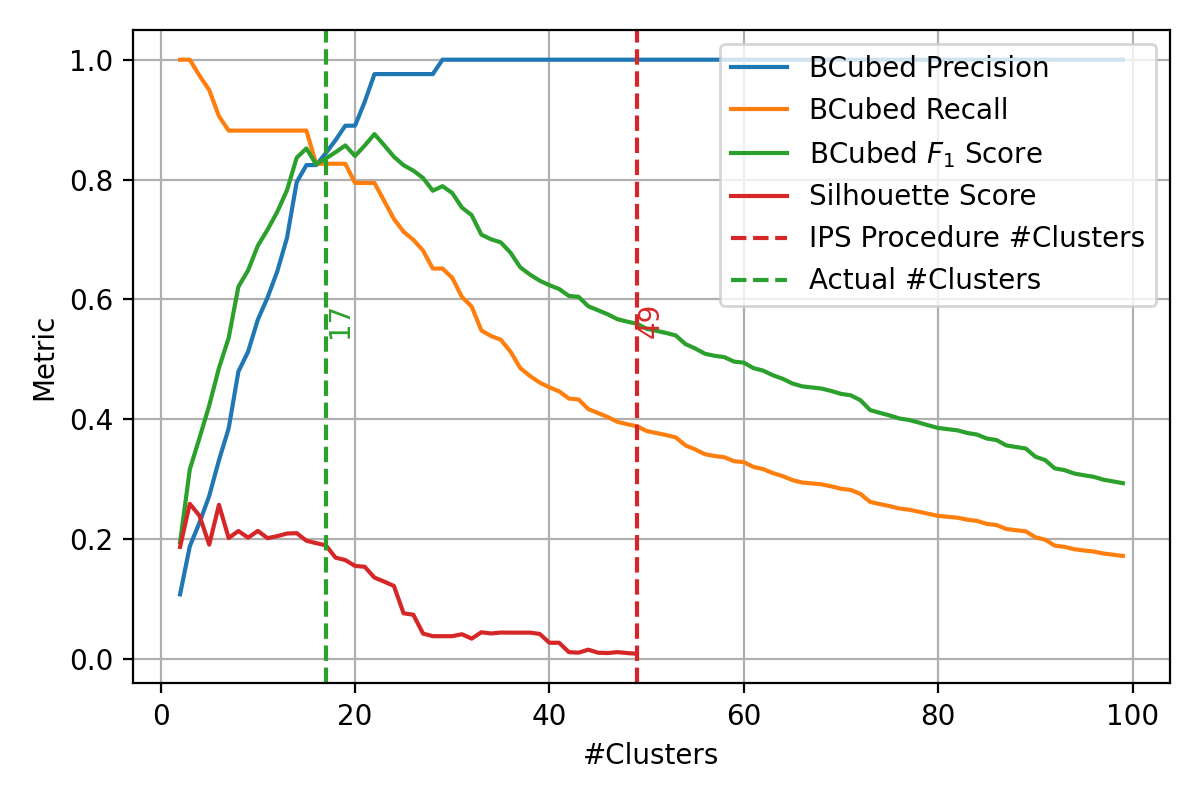
\includegraphics[width=\linewidth]{img/unsupervised_clustering_st_jean_A.png}

  \subcaption{St-Jean B}
  \label{fig:unsupervised_clustering_st_jean_B}
  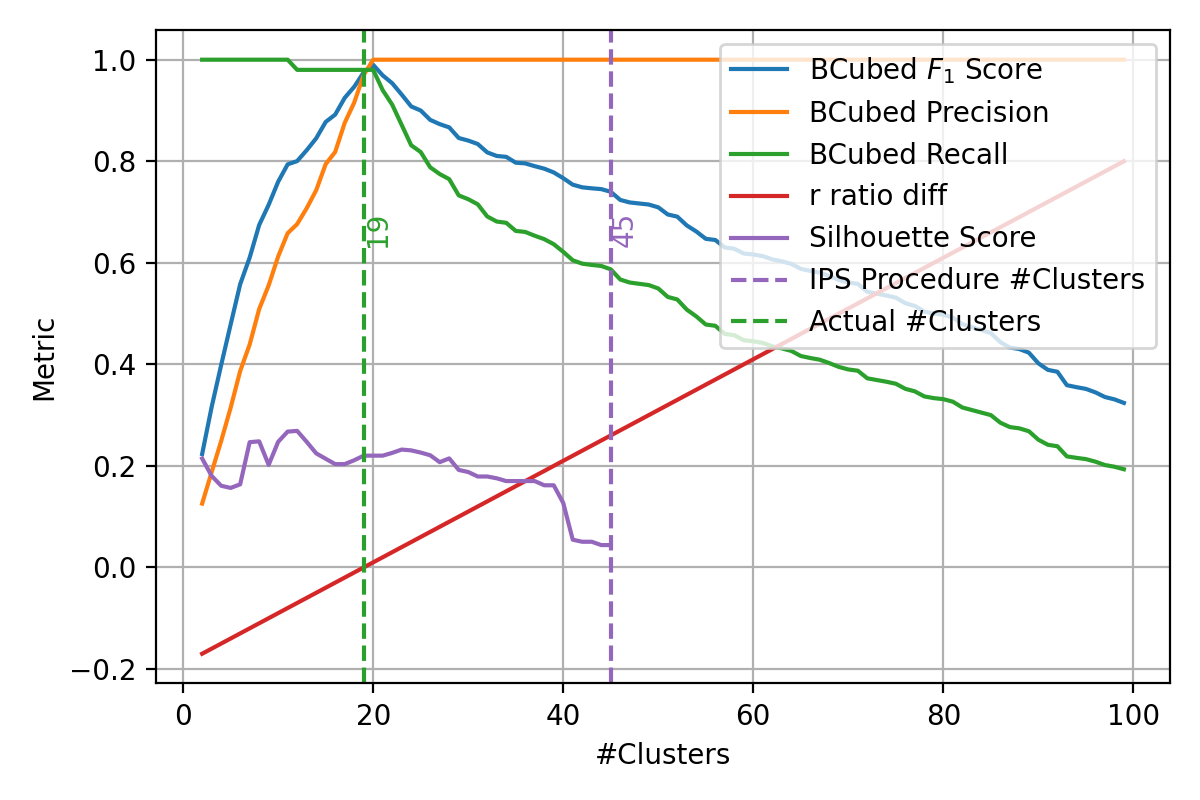
\includegraphics[width=\linewidth]{img/unsupervised_clustering_st_jean_B.png}

  \subcaption{St-Jean}
  \label{fig:unsupervised_clustering_st_jean}
  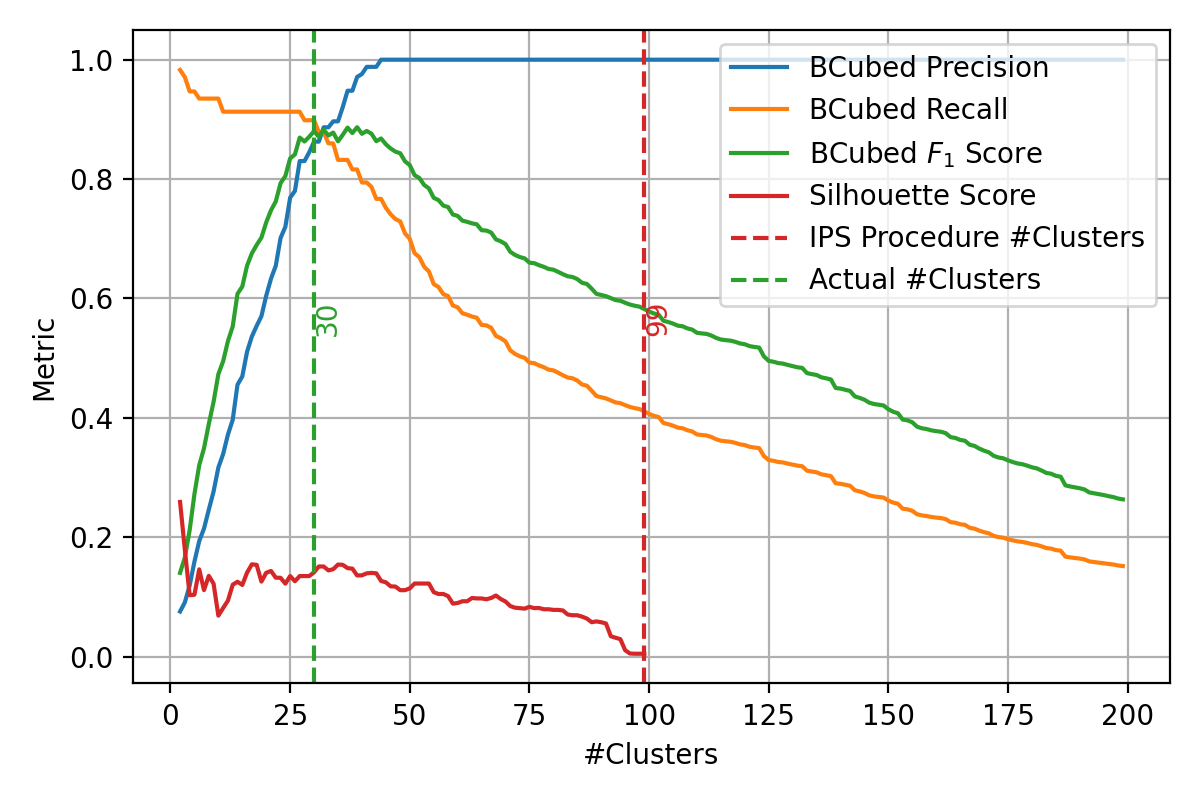
\includegraphics[width=\linewidth]{img/unsupervised_clustering_st_jean.png}
\end{figure}

\subsubsection{Clustering with the supervised cut method}

\begin{table}

  \begin{tabular}{l c c c c c}
    \multicolumn{2}{c}{\multirow{2}{*}{BCubed F1-Score}} & \multicolumn{4}{c}{Testing}\\
    \multicolumn{2}{c}{}                  & Oxquarry & Brunet & St-Jean A & St-Jean B \\
    \parbox[t]{2mm}{\multirow{4}{*}{\rotatebox[origin=c]{90}{Training}}}  & Oxquarry  &          &        &           &           \\
                              & Brunet    &          &        &           &           \\
                              & St-Jean A &          &        &           &           \\
                              & St-Jean B &          &        &           &           \\
  \end{tabular}
\end{table}

\begin{figure}
  \caption{Clustering with the supervised cut method on St-Jean}
  \label{fig:supervised_clustering_sj}

  \subcaption{Training on St-Jean A}
  \label{fig:supervised_clustering_training_st_jean_A}
  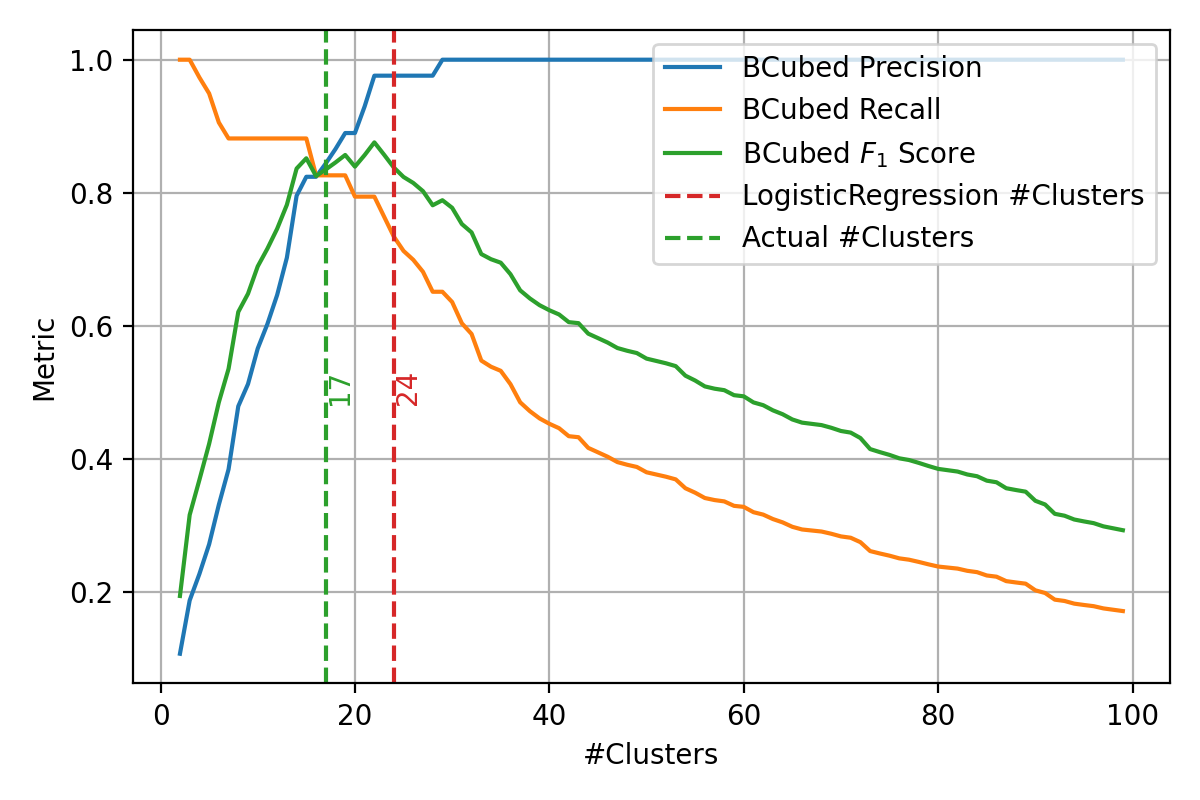
\includegraphics[width=\linewidth]{img/supervised_clustering_training_st_jean_A.png}

  \subcaption{Testing on St-Jean B using the training on St-Jean A}
  \label{fig:supervised_clustering_testing_st_jean_B_with_st_jean_A}
  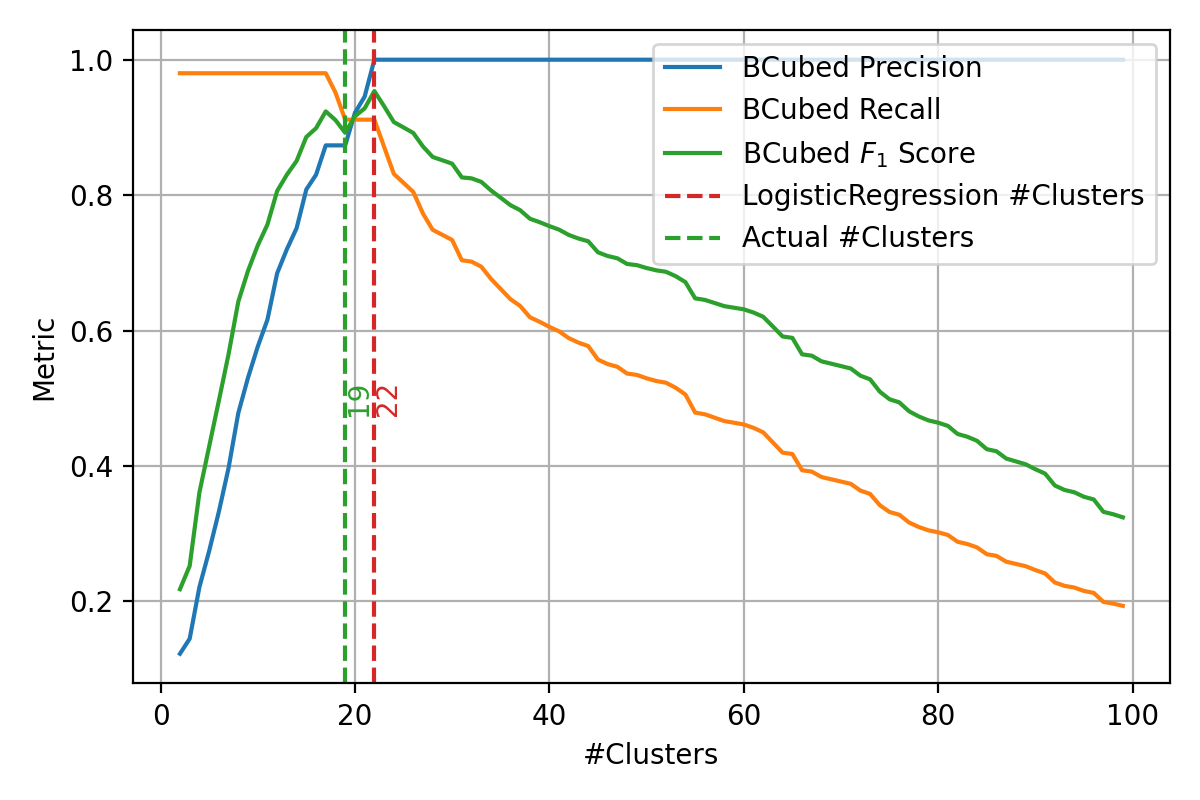
\includegraphics[width=\linewidth]{img/supervised_clustering_testing_st_jean_B_with_st_jean_A.png}
\end{figure}
